\chapter{Numerical ordinary differential equations}
\label{cha:ode}

\minitoc

\section*{Introduction}
This chapter concerns the numerical solution of ordinary differential equations (ODEs) of the following form:
\begin{equation}
    \label{eq:ode}
    \left \{
    \begin{aligned}
        & \vect x'(t) = \vect f\bigl(t, \vect x(t)\bigr), \\
        & \vect x(t_0) = \vect x_0.
    \end{aligned}
    \right.
\end{equation}
Here $\vect f\colon \real \times \real^n \to \real$ and $\vect x_0$ is the initial condition.
Equations of this type
are the building blocks of a plethora mathematical models in science and engineering.
They have applications in celestial dynamics, molecular simulation and fluid mechanics, to mention just a few.
Ordinary differential equations also arise after discretization of time-dependent partial differential equations,
which are also ubiquitous in science.
More often than not,
it is not possible to find an explicit solution of~\eqref{eq:ode},
and so one has to resort to numerical simulation.
The rest of chapter is organized as follows:
\begin{itemize}
    \item
        In \cref{sec:existence},
        we define the concepts of local and global solutions for the continuous-time problem~\eqref{eq:ode},
        and we recall fundamental results concerning the existence and uniqueness of a solution.

    \item
        In~\cref{sec:one-step_methods},
        we analyze the so-called \emph{one-step} numerical methods to solve~\eqref{eq:ode}.
        We emphasize in particular the concepts of \emph{consistency}, \emph{stability} and \emph{convergence}.

    \item
        In~\cref{sec:multistep_methods},
        we present \emph{multistep} methods to solve~\eqref{eq:ode},
        and discuss their drawbacks and advantages compared to one-step methods.

    \item
        Finally, in~\cref{sec:absolute_stability},
        we introduce the concept of \emph{absolute stability} and discuss its relevance in the context of \emph{stiff} differential equations.
\end{itemize}

\section{Analysis of the continuous problem}
A differentiable function $\vect x\colon I \to \real^n$,
where $I$ denotes an interval of $\real$ containing $t_0$,
is a solution of~\eqref{eq:ode} if $\vect x(t_0) = \vect x_0$ and the equation~\eqref{eq:ode} is satisfied for all~$t \in I$.
The solution is called global if~$I = \real$,
and local otherwise.

\paragraph{Integral formulation.}
If $\vect x$ is a solution to~\eqref{eq:ode},
then it holds that
\begin{equation}
    \label{eq:ode_integral}
    \forall  t \in I, \qquad
    \vect x(t) = \vect x_0 + \int_{t_0}^{t} \vect f\bigl(s, \vect x(s)\bigr) \, \d s.
\end{equation}
The converse statement is not true in general,
because a solution to~\eqref{eq:ode_integral} need not necessarily be differentiable everywhere.
However, if the integral formulation~\eqref{eq:ode_integral} holds,
then necessarily $\vect x$ is absolutely continuous
and~\eqref{eq:ode} is satisfied for almost every~$t$.
Additionally, if~\eqref{eq:ode_integral} is satisfied and the function~$\vect f$ is continuous,
then the function~$s \mapsto \vect f\bigl(s, \vect x(s)\bigr)$ is continuous,
and so~\eqref{eq:ode} is satisfied for all $t \in I$ by the fundamental theorem of analysis.
We now focus on the integral formulation~\eqref{eq:ode_integral},
and begin by establishing existence of a local solution.

\label{sec:existence}
\begin{theorem}
    [Existence of a solution]
    \label{theorem:existence}
    Let $\vect x_0 \in \real^n$ and let $\Omega_{\mathcal T, \mathcal R}$ denote the set
    \[
        \bigl\{(t, \vect x) \in \real \times \real^n: \abs{t-t_0} \leq \mathcal T \text{ and } \vecnorm{\vect x - \vect x_0} \leq \mathcal R \bigr\},
    \]
    Assume that the following conditions are satisfied:
    \begin{itemize}
        \item
            The function $\vect f$ is uniformly bounded on~$\Omega_{\mathcal T, \mathcal R}$:
            \begin{equation}
                \label{eq:boundedness_ode}
                \forall (t, \vect x) \in \Omega_{\mathcal T, \mathcal R}, \qquad
                \vecnorm{\vect f(t, \vect x)} \leq M.
            \end{equation}

        \item
            The function $\vect f$ satisfies the following Lipschitz condition:
            there is $L > 0$ such that
            \begin{equation}
                \label{eq:local_lipschitz_ode}
                \forall \bigl((t, \vect x_1), (t, \vect x_2)\bigr) \in \Omega_{\mathcal T, \mathcal R} \times \Omega_{\mathcal T, \mathcal R}, \qquad
                \vecnorm{ \vect f(t, \vect x_1) - \vect f(t, \vect x_2) } \leq L \vecnorm{\vect x_1 - \vect x_2}.
            \end{equation}
    \end{itemize}
    Then there exists $T \in (0, \mathcal T]$ depending on $\mathcal R$, $M$ and $L$ such that
    the differential equation~\eqref{eq:ode_integral} has a local solution $\vect x\colon [t_0 - T, t_0 + T] \to \real^n$.
\end{theorem}
\begin{proof}
    Fix $T \in (0, \mathcal T]$ and let $I = [t_0 - T, t_0 + T]$.
    Let also $\mathcal X$ denote the following subset of continuous functions defined from~$I$ to $\real^n$:
    \[
    \mathcal X := \left\{ \vect x\in C\left(I, \real^n\right) : \sup_{t \in I} \norm[\big]{\vect x(t) - \vect x_0} \leq \mathcal R \right\}
    \]
    The set~$\mathcal X$ endowed with supremum metric is a closed subset of~$C(I, \real^n)$.
    Since $\mathcal X$ is a closed subset of a complete metric space,
    it is itself complete.
    Let $\Phi \colon \mathcal X \to C(I, \real^n)$ denote the mapping
    \[
        \Phi(\vect x) \colon  t \mapsto  \vect x_0 + \int_{0}^{t} \vect f\bigl(s, \vect x(s)\bigr) \, \d s.
    \]
    The right-hand side, being the integral of a bounded function,
    is indeed a continuous function.
    We will show that, for~$T$ sufficiently small,
    \begin{itemize}
        \item the mapping $\Phi$ maps $\mathcal X$ into $\mathcal X$;
        \item the mapping $\Phi$ is a contraction.
    \end{itemize}
    From~\eqref{eq:boundedness_ode},
    it follows that
    \[
        \forall \vect x \in \mathcal X, \qquad
        \forall t \in I, \qquad
        \vecnorm*{\Phi(\vect x)(t) - \vect x_0} = \vecnorm*{ \int_{t_0}^{t} \vect f\bigl(s, \vect x(s)\bigr) \, \d s }
        \leq M T.
    \]
    On the other hand, from the Lipschitz condition~\eqref{eq:local_lipschitz_ode},
    it holds that
    \[
        \forall (\vect x, \vect y) \in \mathcal X \times \mathcal X, \qquad
        \norm{\Phi(\vect x) - \Phi(\vect y)} \leq L T \norm{\Phi(\vect x) - \Phi(\vect y)}.
    \]
    Therefore, it suffices to take $T < \min \left\{ \mathcal T, \frac{\mathcal R}{M}, \frac{1}{L} \right\}$ to ensure that the above conditions are satisfied.
    For a value of~$T$ in this range,
    the Banach fixed point theorem, \cref{theorem:banach_fixed_point},
    gives the existence of a unique fixed point~$\vect x_* \in \mathcal X$ of~$\Phi$.
    Since a fixed point of~$\Phi$ is a solution to~\eqref{eq:ode_integral} in view of the definition of~$\Phi$,
    the statement is proved.
\end{proof}
It may seem at first glance that uniqueness of the solution to~\eqref{eq:ode_integral} follows from the uniqueness of the fixed point guaranteed by~\cref{theorem:banach_fixed_point}.
However, this theorem implies uniqueness \emph{only in the set~$\mathcal X$},
a property known as~\emph{conditional uniqueness}.
In order to prove that the solution is unique over the full space $C([t_0-T, t_0+T], \real^n)$,
additional assumptions and arguments are required.
A simple approach is to rely on Gr\"onwall's lemma.
\begin{lemma}
    [Gr\"onwall's lemma, simplified integral form]
    Suppose that $u \colon [t_0-T, t_0+T] \to \real_{\geq 0}$ is continuous, nonnegative, and satisfies
    \begin{equation}
        \label{eq:gronwall_condition}
        \forall t \in [t_0, t_0+T], \qquad
        u(t) \leq \alpha + \int_{t_0}^{t} \beta(s) \, u(s) \, \d s,
    \end{equation}
    where $\alpha \geq 0$ and $\beta\colon [t_0, t_0 + T] \to \real_{\geq 0}$ is continuous and nonnegative.
    Then
    \begin{equation}
        \label{eq:gronwall}
        \forall t \in [t_0, t_0+T], \qquad
        u(t) \leq \alpha \exp \left( \int_{t_0}^{t} \beta(s) \, \d s \right).
    \end{equation}
\end{lemma}
\begin{proof}
    Assume first that~$\alpha > 0$,
    so that the logarithm in~\eqref{eq:intermediate_gronwall} is well-defined.
    By the fundamental theorem of calculus and~\eqref{eq:gronwall_condition},
    it holds that
    \[
        \frac{\d}{\d t} \left( \alpha + \int_{t_0}^{t} \beta(s) \, u(s) \, \d s \right)
        \leq \beta(t) \left( \alpha + \int_{t_0}^{t} \beta(s) \, u(s) \, \d s \right)
    \]
    Therefore we have
    \begin{equation}
        \label{eq:intermediate_gronwall}
        \frac{\d}{\d t} \log \left( \alpha + \int_{t_0}^{t} \beta(s) \, u(s) \, \d s \right) \leq \beta(t),
    \end{equation}
    and after integrating and exponentiating,
    we obtain
    \[
        \alpha + \int_{t_0}^{t} \beta(s) \, u(s) \, \d s
        \leq \alpha \exp \left( \int_{t_0}^{t} \beta(s) \, \d s \right)
    \]
    The statement then follows by using~\eqref{eq:gronwall_condition} again.
    Assume next that $\alpha = 0$.
    If~\eqref{eq:gronwall_condition} is satisfied for~$\alpha = 0$,
    then this condition is also satisfied for all $\alpha > 0$.
    Therefore the conclusion~\eqref{eq:gronwall} holds for all~$\alpha > 0$,
    and taking the limit $\alpha \to 0$ in this equation,
    we obtain the statement.
\end{proof}
Note that the estimate~\eqref{eq:gronwall} is sharp,
since the function $v \colon [t_0, t_0 + T]$ given by
\[
    v(t) = \alpha \exp \left( \int_{t_0}^{t} \beta(s) \, \d s \right)
\]
satisfies~\eqref{eq:gronwall_condition} with equality.
We are now ready to prove uniqueness under an appropriate condition.
\begin{theorem}
    [Uniqueness of the solution]
    \label{theorem:uniqueness}
    Let $\vect x_0 \in \real^n$ and let
    \[
        \Omega_{\mathcal T, \mathcal R}
        \bigl\{(t, \vect x) \in \real \times \real^n: \abs{t - t_0} \leq \mathcal T \text{ and } \vecnorm{\vect x - \vect x_0} \leq \mathcal R \bigr\},
    \]
    Assume that for all $\mathcal T \in \real_{>0}$ and $\mathcal R \in \real_{>0}$,
    there is $L_{\mathcal T,  \mathcal R}$ such that
    \begin{equation}
        \label{eq:local_lipschitz_uniqueness}
        \forall \bigl((t, \vect x_1), (t, \vect x_2)\bigr) \in \Omega_{\mathcal T, \mathcal R} \times \Omega_{\mathcal T, \mathcal R}, \qquad
        \vecnorm{ \vect f(t, \vect x_1) - \vect f(t, \vect x_2) } \leq L_{\mathcal T, \mathcal R} \vecnorm{\vect x_1 - \vect x_2}.
    \end{equation}
    Then if $\vect x_1$ and $\vect x_2$ in $C\bigl([t_0 - T, t_0 + T], \real^n\bigr)$ are local solutions to~\eqref{eq:ode_integral},
    it holds that $\vect x_1 = \vect x_2$.
\end{theorem}
\begin{proof}
    Suppose that $\vect x_1$ and $\vect x_2$ are solutions to~\eqref{eq:ode_integral}.
    Let~$I = [t_0 - T, t_0 + T]$ and
    \[
        R := \max \left\{ \sup_{t \in I} \norm{\vect x_1(t) - \vect x_0},   \sup_{t \in I} \norm{\vect x_2(t) - \vect x_0} \right\} < \infty,
    \]
    Since $\vect x_1$ and $\vect x_2$ are solutions,
    it holds that
    \[
        \forall t \in [t_0 - T, t_0 + T], \qquad
        \vect x_1(t) - \vect x_2(t) = \int_{t_0}^{t} \Bigl( f\bigl(s, \vect x_1(s)\bigr) - f\bigl(s, \vect x_2(s)\bigr) \Bigr)  \, \d s.
    \]
    Taking the norm and using~\eqref{eq:local_lipschitz_uniqueness},
    we obtain
    \[
        \forall t \in [t_0, t_0 + T], \qquad
        \vecnorm{\vect x_1(t) - \vect x_2(t)} \leq L_{T,R} \int_{t_0}^{t} \vecnorm{\vect x_1(s) - \vect x_2(s)} \, \d s
    \]
    Using Gr\"onwall's lemma,
    we deduce that~$\vect x_1(t) = \vect x_2(t)$ for all $t \in [t_0, t_0 + T]$.
    A similar argument can be employed to show that $\vect x_1 = \vect x_2$ on $[t_0 - T, t_0]$.
\end{proof}

\begin{corollary}
    [Maximal solutions]
    \label{corollary:maximal_solutions}
    Assume that $\vect f$ is continuous in~$t$ and satisfies the local Lipschitz condition~\eqref{eq:local_lipschitz_uniqueness}.
    Then there exists $- \infty \leq T_- < T_+ \leq \infty$ such that $t_0 \in (T_-, T_+)$ and
    the following properties are satisfied.
    \begin{itemize}
        \item
            there exists a solution $\vect x_* \colon (T_-, T_+) \to \real^n$ to~\eqref{eq:ode_integral};

        \item
            if $\vect x\colon I \to \real^n$ is a local solution of~\eqref{eq:ode_integral},
            then $I \subset (T_-, T_+)$ and $\vect x(t) = \vect x_*(t)$ for all~$t \in I$.

        \item
            If $T_+$ is finite, then $\lim_{t \to T_+} \vecnorm[\big]{\vect x(t)} = \infty$,
            and if $T_-$ is finite,
            then $\lim_{t \to T_-} \vecnorm[\big]{\vect x(t)} = \infty$.
    \end{itemize}
    The solution $\vect x_*$ is called the maximal solution of~\eqref{eq:ode_integral}.
\end{corollary}
\begin{proof}
    Let $\mathcal I$ denote the union of all the open intervals~$I$ such that there exists a solution in~$C(I, \real^n)$ to~\eqref{eq:ode_integral}.
    The open set $\mathcal I$ is connected and, by~\cref{theorem:existence},
    it contains a neighborhood of~$t_0$.
    Therefore $\mathcal I$ is of the form $(T_-, T_+)$,
    where $-\infty \leq T_- <  t_0 < T_+ \leq \infty$.
    In view of~\cref{theorem:uniqueness},
    all the local solutions coincide where they are defined,
    and so they can be patched together in order to construct a solution~$\vect x_*\colon (T_-, T_+) \to \real$.
    It remains to prove the third item.
    To this end, suppose for contradiction that $T_+$ was finite and that
    there was $(t_n)_{n \in \nat}$ such that $t_n \to T_+$ in the limit~$n \to \infty$ and~
    \[
        K := \sup_{n \in \nat} \vecnorm{\vect x_*(t_n)} < \infty.
    \]
    Since $\vect f$ is continuous,
    there is $M$ such that $\lvert f(t, \vect x) \rvert$ is uniformly bounded from above by~$M$ for all $(t, \vect x) \in [T_- - 1, T_+ + 1] \times B_{K+1}(\vect 0)$.
    Furthermore, by the assumption~\eqref{eq:local_lipschitz_uniqueness},
    there is $L$ such that for all $t \in [T_- - 1, T_+ + 1]$,
    the following Lipschitz condition holds:
    \[
        \forall (\vect x_1, \vect x_2) \in  B_{K+1}(\vect 0) \times B_{K+1}(\vect 0), \qquad
        \vecnorm{ \vect f(t, \vect x_1) - \vect f(t, \vect x_2) } \leq L \vecnorm{\vect x_1 - \vect x_2}.
    \]
    Consequently, \cref{theorem:existence} with $\mathcal T = \mathcal R = 1$ implies for all~$n$ the existence of a solution to
    \[
        \left \{
        \begin{aligned}
            & \vect x'(t) = \vect f\bigl(t, \vect x(t)\bigr), \\
            & \vect x(t_n) = \vect x_*(t_n).
        \end{aligned}
        \right.
    \]
    over the time interval $[t_n - T, t_n + T]$, where $T > 0$ depends only on $M$ and $L$, and not on~$n$.
    But then, for~$n$ sufficiently large,
    this solution extends beyond $T_+$,
    which contradicts the maximality of~$\mathcal I$.
    An analogous reasoning can be employed for~$T_-$.
\end{proof}
\begin{example}
    Consider the ODE
    \[
        \left \{
        \begin{aligned}
            & x'(t) = x(t)^2, \\
            & x(0) = 1.
        \end{aligned}
        \right.
    \]
    The maximal solution is $x_* \colon (-\infty, 1) \to \real$ given by
    \[
        \vect x_*(t) = \frac{1}{1-t}.
    \]
\end{example}

\paragraph{Existence of a unique global solution.}
In certain settings,
it is possible to prove the maximal solution to~\eqref{eq:ode_integral} is globally defined for any initial condition.
We discuss a few important examples.
\begin{itemize}
    \item
        The first case is when $\vect f\colon \real \times \real^n$ is globally Lipschitz in its second argument,
        with a Lipschitz constant that depends continuously on the first argument.

    \item
        The second case,
        generalizing the first,
        is when the growth of~$\vect f(t, \placeholder)$ is at most affine:
        \[
            \forall (t, \vect x) \in \real \times \real^n, \qquad
            \vecnorm{ \vect f(t, \vect x) } \leq C(t) + L(t) \vecnorm{ \vect x },
        \]
        with continuous constants~$C(t)$ and $L(t)$.

    \item
        The third case is when $\vect f$ is independent of~$t$ and there is a function~$W \in C^1(\real^n)$ such that~$W(\vect x) \to \infty$ in the limit as $\vecnorm{\vect x} \to \infty$
        and
        \[
            \forall \vect x \in \real^n, \qquad
            \nabla W(\vect x) \cdot \vect f(\vect x) \leq c < \infty
        \]
        Such a function is called a \emph{Lyapunov function}.
\end{itemize}
The strategy of proof for global existence usually relies on an argument by contradiction.
Consider for example the third setting.
Since the assumptions of~\cref{corollary:maximal_solutions} are satisfied,
there exists a maximal solution $\vect x_*\colon (T_-, T_+) \to \infty$.
Assume for contradiction that~$T_+$ is finite.
Then the third item in~\cref{corollary:maximal_solutions} implies that $\lim_{t \to T_+} \vecnorm{\vect x_*(t)} \to \infty$,
and so~$W\bigl(\vect x_*(t)\bigr)$ blows up as~$t$ approaches $T^+$.
On the other hand, we have
\[
    \frac{\d}{\d t} W\bigl(\vect x_*(t)\bigr) = \nabla W\bigl(\vect x_*(t)\bigr) \cdot \vect f\bigl(\vect x_*(t)\bigr) \leq c.
\]
Therefore $\lim_{t \to T_+} W\bigl(\vect x_*(t)\bigr) \leq W\bigl(\vect x_*(t_0)\bigr) + \lvert c \rvert (T_+ - t_0)$,
which is a contradiction.

% \paragraph{Lyapunov stability.}
% Before we move to the study of numerical schemes for SDEs,
% we introduce one last important concept: that of \emph{Lyapunov stability}.
% To precisely define this concept,
% Suppose that the assumptions of~\cref{corollary:maximal_solutions} are satisfied and
% consider the differential equation~\eqref{eq:ode} over an interval~$[-T, T]$,
% with $T_- < -T < T < T_+$, and the following perturbation thereof:
% \begin{equation}
%     \label{eq:ode_perturbed}
%     \left \{
%     \begin{aligned}
%         & \dot {\vect x_{\delta}}(t) = \vect f\bigl(t, \vect x(t)\bigr) + \vect \delta\bigl(t, \vect x(t)\bigr), \\
%         & \vect x_{\delta}(t_0) = \vect x_0 + \vect \delta_0.
%     \end{aligned}
%     \right.
% \end{equation}
% Roughly speaking, Lyapunov stability is a property of the differential equation which
% guarantees that the solution to the perturbed equation~\eqref{eq:ode_perturbed} remains close to that of the unperturbed equation~\eqref{eq:ode}
% when the perturbation is small.
% \begin{definition}
%     [Stability in the sense of Lyapunov]
%     Equation~\eqref{eq:ode} is stable in the sense of Lyapunov if there is $C = C(T)$ such that
%     for all~$\varepsilon > 0$ and all $\vect \delta \colon \real \times \real^n \to \real$ continuous and bounded and all $\vect \delta_0$ with
%     \[
%         \sup_{(t, \vect x) \in [-T, T] \times \real^d} \vecnorm{ \vect \delta(t, \vect x)} \leq \varepsilon
%         \quad \text{ and } \quad
%         \vecnorm{\vect \delta_0} \leq \varepsilon
%     \]
% \end{definition}

\section{One-step methods}
\label{sec:one-step_methods}
From now on, we assume for simplicity that $t_0 = 0$ and that
the initial value problem~\eqref{eq:ode} admits a unique solution over the interval $[0, T]$.
Most numerical methods for ODEs construct an approximation of the solution at discrete points:
\[
    \vect x_n \approx \vect x(t_n), \qquad n = 0, 1, 2, \dotsc.
\]
The discretization points $(t_n)_{n \in \nat}$ are commonly equidistant,
i.e.~$t_n = n \Delta$ where $\Delta$ is the \emph{discretization step}.
Sometimes, it is useful to employ a variable time step,
but we assume throughout this section that the time step is fixed, for simplicity.
We begin in~\cref{sub:explicit_euler} and~\cref{sub:implicit_euler} by studying the simplest one-step methods,
namely the forward and backward Euler methods.
Then, in~\cref{sub:one_step_general},
we present a general approach to the analysis of one-step methods.
Finally, in~\cref{sub:other_one_step},
we present other widely used one-step methods in applications.

\subsection{Forward Euler method}
\label{sub:explicit_euler}
Assume that~\eqref{eq:ode} has a unique solution~$\vect x(t)$ over the interval $[0, T]$.
If $\vect x(t)$ is twice continuously differentiable,
then by Taylor's formula,
we have
\begin{equation}
    \label{eq:taylor_forward}
    \vect x(t + \Delta) = \vect x(t) + \Delta \vect f(t, \vect x) + \frac{\Delta^2}{2} \vect x''(\tau),
    \qquad \tau \in (t, t+\Delta).
\end{equation}
This motivates a method known as the \emph{forward} or \emph{explicit} Euler method:
\[
    \vect x_{n+1} = \vect x_{n} + \Delta \vect f(t_n, \vect x_n),
\]
with the same initial condition as for the continuous equation~\eqref{eq:ode}.
The convergence of this method can be proved under a global Lipschitz assumption on the function~$\vect f$.

\begin{theorem}
    [Convergence of the forward Euler method]
    \label{theorem:forward_euler}
    Assume that there is $L \in \real_{>0}$ such that
    \begin{equation}
        \label{eq:global_lipschitz}
        \forall (t, \vect x, \vect y) \in \real \times \real^n \times \real^n, \qquad
        \vecnorm{\vect f(t, \vect x) - \vect f(t, \vect y)}
        \leq L \vecnorm{\vect x - \vect y}.
    \end{equation}
    Suppose in addition that there exists a unique, twice continuously differentiable of~\eqref{eq:ode} over the interval~$[0, T]$,
    and let
    \[
        M = \sup_{t \in [0,T]} \vecnorm{\vect x''(t)}
    \]
    Then the following error estimate holds:
    \begin{equation}
        \label{eq:error_bound_forward_euler}
        \forall n \in \left\{0, 1, \dotsc, \floor*{\frac{T}{\Delta}} \right\},
        \qquad
        \vecnorm{\vect x(t_n) - \vect x_n}
        \leq
        \frac{\Delta M}{2} \left( \frac{\e^{L t_n} - 1}{L} \right).
    \end{equation}
\end{theorem}
\begin{proof}
    Notice that
    \begin{align*}
        \vect x(t_{n}) - \vect x_{n}
        &= \left( \vect x(t_{n-1}) + \Delta \, \vect f\bigl(t_{n-1}, \vect x(t_{n-1})\bigr) + \frac{\Delta^2}{2} \vect x''(\tau_n) \right)
        - \Bigl( \vect x_{n-1} + \Delta \, \vect f\bigl(t_{n-1}, \vect x_{n-1}\bigr) \Bigr) \\
        &= \bigl(\vect x(t_{n-1}) - \vect x_{n-1}\bigr) + \Delta \Bigl( \vect f\bigl(t_{n-1}, \vect x(t_{n-1})\bigr) - \vect f\bigl(t_{n-1}, \vect x_{n-1}\bigr) \Bigr) + \frac{\Delta^2}{2} \vect x''(\tau_n),
    \end{align*}
    for some $\tau_n \in (t_{n-1}, t_n)$.
    Let $\vect e_n = \vect x(t_n) - \vect x_n$ and $\vect \varepsilon_n = \frac{\Delta^2}{2} \vect x''(\tau_n)$.
    The first term is the error at iteration~$n-1$,
    and the second may be bounded from~\eqref{eq:global_lipschitz},
    which gives
    \begin{align*}
        \vecnorm{\vect e_{n}}
        &\leq (1 + \Delta L) \vecnorm{\vect e_{n-1}}
        + \vecnorm{\vect \varepsilon_n}.
    \end{align*}
    The structure of this equation is important,
    as it appears in the analysis of all one-step methods for ODEs.
    The first term is an amplification of the error at the previous iteration,
    and the second term is an upper bound on the additional error introduced at step~$n$.
    Applying this inequality to the previous time steps, we obtain
    \begin{align}
        \nonumber
        \vecnorm{\vect e_{n}}
        &\leq (1 + \Delta L) \Bigl( (1 + \Delta L) \vecnorm{\vect e_{n-2}} + \vecnorm{\vect \varepsilon_{n-1}} \Bigr) + \vecnorm{\vect \varepsilon_{n}} \\
        \label{eq:sum_local_and_accumulation}
        &\leq \dotsc
        \leq (1 + \Delta L)^{n} \vecnorm{\vect e_{0}} + \sum_{i=1}^{n} (1 + \Delta L)^{n-i} \vecnorm{\vect \varepsilon_{i}}.
    \end{align}
    Since $\vecnorm{\vect \varepsilon_i} \leq \Delta^2M/2$,
    we have by using the formula for geometric series that
    \[
        \vecnorm{\vect e_{n}}
        \leq (1 + \Delta L)^{n} \vecnorm{\vect e_{0}} + \frac{(1+\Delta L)^{n} - 1}{\Delta L} \left( \frac{\Delta^2 M}{2} \right).
    \]
    The first term is zero because $\vecnorm{\vect e_{0}} = 0$.
    Using the bound $(1+\Delta L)^n \leq \bigl(\exp(\Delta L)\bigr)^n = \e^{L t_n}$ in the second term and rearranging,
    we finally obtain the statement~\eqref{eq:error_bound_forward_euler}.
\end{proof}

\subsection{Backward Euler method}
\label{sub:implicit_euler}
If we apply the Taylor expansion~\eqref{eq:taylor_forward} backward around~$t + \Delta$,
instead of forward around~$t$,
then we obtain
\[
    \label{eq:taylor_backward}
    \vect x(t) = \vect x(t + \Delta) - \Delta \vect f(t + \Delta, \vect x) + \frac{\Delta^2}{2} \vect x''(\tau),
    \qquad \tau \in (t, t+\Delta).
\]
This motivates the so-called \emph{backward} or \emph{implicit} Euler method:
\begin{equation}
    \label{eq:backward_euler}
    \vect x_{n+1} = \vect x_{n} + \Delta \vect f(t_{n+1}, \vect x_{n+1}).
\end{equation}
Observe that the right-hand side depends on $\vect x_{n+1}$.
Therefore, given $t_n$ and $\vect x_n$,
this is a nonlinear equation for the unknown $\vect x_{n+1}$,
which can be solved by using any of the methods studied in~\cref{cha:solution_of_nonlinear_systems}.
Finding a solution to~\eqref{eq:backward_euler} amounts to finding a fixed point of the function
\[
    \vect y \mapsto \vect F(\vect y) := \vect x_{n} + \Delta \vect f(t_n, \vect y).
\]
A priori, the existence and uniqueness of such a fixed point is not guaranteed.
We proved in~\cref{theorem:exponential_convergence_fixed_point} that a sufficient condition for these two properties to hold is
that~$\vect F$ is globally Lipschitz with a constant strictly less than 1,
which holds if and only if the function~$\vect y \mapsto \vect f(t_n, \vect y)$ is globally Lipschitz with a constant strictly less than $1/\Delta$.
If the condition~\eqref{eq:global_lipschitz} holds, for example,
then the backward Euler method~\eqref{eq:backward_euler} is guaranteed to be well defined for $\Delta < \frac{1}{L}$.
\Cref{theorem:exponential_convergence_fixed_point} also ensures that, if~$\vect F$ is globally Lipschitz with a constant less than~$1$,
then the fixed point can be approximated by using the iteration
\begin{equation}
    \label{eq:fixed_point_ode}
    \vect y_{k+1} = \vect F(\vect y_k).
\end{equation}
and there is exponential convergence~$\vect y_k \to \vect x_{n+1}$ in the limit as $k \to \infty$.
A natural starting point for~\eqref{eq:fixed_point_ode} is~$\vect y_0 = \vect x_n$.
An alternative approach to the fixed point iteration~\eqref{eq:fixed_point_ode} is to use the Newton--Raphson method for~\eqref{eq:backward_euler},
which is faster in principle but must be initialized sufficiently close to the fixed point.

Using a reasoning similar to that employed for proving~\cref{theorem:forward_euler},
we can prove the following result.
\begin{theorem}
    [Convergence of the backward Euler method]
    If the assumptions of~\cref{theorem:forward_euler} hold and $\Delta < \frac{1}{L}$,
    then the following error estimate holds:
    \begin{equation}
        \label{eq:estimate_backward_euler}
        \forall n \in \left\{0, 1, \dotsc, \floor*{\frac{T}{\Delta}} \right\},
        \qquad
        \vecnorm{\vect x(t_n) - \vect x_n}
        \leq
        \frac{\Delta M}{2} \left( \frac{\left( \frac{1}{1 - \Delta L} \right)^n - 1}{L} \right).
    \end{equation}
\end{theorem}
\begin{proof}
    The proof is left as an exercise.
\end{proof}
\begin{remark}
    Note that, if $\Delta < \frac{1}{2L}$,
    then
    \begin{align*}
         \frac{1}{1 - \Delta L}
         &= 1 + \Delta L + (\Delta L)^2 + (\Delta L)^3 + (\Delta L)^4 \dotsc \\
         &\leq 1 + \Delta L + (\Delta L)^2 + \frac{1}{2} (\Delta L)^2 + \frac{1}{4} (\Delta L)^2 + \dotsc \\
         &\leq 1 + \Delta L + 2 (\Delta L)^2 \leq \exp\bigl(\Delta L + (\Delta L)^2\bigr),
     \end{align*}
     and so the error estimate~\eqref{eq:estimate_backward_euler} gives
     \[
        \vecnorm{\vect x(t_n) - \vect x_n}
        \leq
        \frac{\Delta M}{2} \left( \frac{\exp(L t_n + \Delta L^2 t_n) - 1}{L} \right),
     \]
     which makes it clear that the right-hand side of~\eqref{eq:estimate_backward_euler} is close,
     in absolute and relative terms, to that of~\eqref{eq:error_bound_forward_euler} when $\Delta \ll 1$.
\end{remark}
At this point, the reader may be wondering why one would use the backward Euler method instead of the forward Euler method,
given that both methods have same order of convergence but iterations of the former are more computationally costly.
The reason is that the backward Euler method,
like many implicit methods,
is more \emph{stable} than its forward counterpart.
Implicit methods are especially attractive in the context of~\emph{stiff} differential equations.
We shall elaborate on this subject in~\cref{sec:absolute_stability}.

\subsection{Analysis of general one-step methods}
\label{sub:one_step_general}
In general, one-step methods to solve differential equations are of the abstract form
\begin{equation}
    \label{eq:general_one_step}
    \vect x_{n+1} = \vect x_n + \Delta \vect \Phi_{\Delta}(t_n, \vect x_n).
\end{equation}
where $\vect \Phi_{\Delta}\colon \real \times \real^n \to \real^n$ is a function such that
\begin{equation}
    \label{eq:one_step_integral}
    \vect \Phi_{\Delta}(t, \vect x)
    \approx \frac{1}{\Delta} \int_{t}^{t+\Delta} \vect f\bigl(s, \vect x^{t, \vect x}(s)\bigr) \, \d s
    = \frac{\vect x^{t, \vect x}(t + \Delta) - \vect x}{\Delta}.
\end{equation}
Here $\vect x^{t, \vect x}$ denotes the solution to the differential equation~\eqref{eq:ode} with initial condition $\vect x(s) = \vect x$.
The main goal of this section is to establish general conditions,
known as \emph{consistency} and \emph{stability},
under which the numerical scheme~\eqref{eq:general_one_step} is convergent.
As we observed in the proof of~\cref{theorem:forward_euler}
-- specifically in equation~\eqref{eq:sum_local_and_accumulation} --
the error at the final iteration for the forward Euler method is a sum of local errors,
each amplified by a factor depending to the number of iterations left to reach the final time.
\emph{Consistency} of a numerical method enables to control the size of local errors when they arise,
while~\emph{stability} enables to control their growth.

We emphasize that both the forward and the backward Euler methods can be recast in the form~\eqref{eq:general_one_step}.
For the forward Euler method $\vect \Phi_{\Delta}(t, \vect x) = \vect f(t, \vect x)$,
while for the backward Euler method, the function $\vect \Phi_{\Delta}$ is defined implicitly as the function which to~$(t, \vect x)$ associates the solution~$\vect \phi \in \real^n$ to the equation
\[
    \vect \phi = \vect f(t + \Delta, \vect x + \Delta \vect \phi).
\]
\subsubsection*{Local truncation error and consistency}%
The local truncation error is the residual error obtained when substituting the exact solution of the differential equation in~\eqref{eq:general_one_step}:
\[
    \vect \eta_{n+1} := \frac{\vect x(t_{n+1}) - \vect x(t_n)}{\Delta} + \vect \Phi_{\Delta}\bigl(t_n, \vect x(t_n)\bigr).
\]
Since there is a division by~$\Delta$, the local truncation error has the same physical dimension as that of $\vect x'$,
and so it should be viewed as an error \emph{per time unit}.

\begin{definition}
    [Consistency]
    A numerical method is consistent if
    \[
        \lim_{\Delta \to 0} \left( \max_{1 \leq n \leq N} \vecnorm {\vect \eta_n} \right) = 0, \qquad N = \floor*{\frac{T}{\Delta}}.
    \]
    It is consistent with order~$p$ if there exists~$C$ such that
    \[
        \forall \Delta > 0, \qquad
         \max_{1 \leq n \leq N} \vecnorm {\vect \eta_n} \leq C \Delta^p.
    \]
\end{definition}
Proving the consistency of a numerical method is usually achieved on a case-by-case basis by application of Taylor's formula.

\subsubsection*{Stability}%
\label{ssub:Stability}
The stability of a numerical method qualifies its sensitivity to perturbations.
Roughly speaking, it expresses that small perturbation of the right-hand side of~\eqref{eq:general_one_step} lead to small perturbations of the numerical solution.
\begin{definition}
    [Stability]
    A numerical method of the form~\eqref{eq:general_one_step} is stable if there exists a constant~$S(T) > 0$ independent of $\Delta$ such that for all sequence~$(\vect y_n)_{1\leq n \leq N}$ satisfying
    \begin{equation}
        \label{eq:general_one_step_perturbed}
        \vect y_{n+1} = \vect y_n + \Delta \vect \Phi_{\Delta}(t_n, \vect y_n) + \Delta \vect \delta_{n+1}, \qquad \vect y_0 = \vect x_0,
    \end{equation}
    it holds that
    \begin{equation}
        \label{eq:stability_numerical_method}
        \max_{1\leq n \leq N} \vecnorm{ \vect x_n - \vect y_n } \leq S(T) \Delta \sum_{n=1}^{N} \vecnorm{ \vect \delta_n }.
    \end{equation}
\end{definition}
It is convenient to introduce the following norms for sequences of vectors $(\vect u_{n})_{1 \leq n \leq N}$:
\[
    \norm{\vect u_{\placeholder}}_{\ell^1_T} = \sum_{n=1}^{N} \vecnorm{\vect u_{n}},
    \qquad
    \norm{\vect u_{\placeholder}}_{\ell^{\infty}_T} = \max_{1\leq n \leq N} \vecnorm{\vect u_{n}},
\]
With these notations, equation~\eqref{eq:stability_numerical_method} may be rewritten compactly as follows:
\[
    \norm{ \vect x_{\placeholder} - \vect y_{\placeholder} }_{\ell^{\infty}_T} \leq S(T) \Delta \norm{ \vect \delta_{\placeholder} }_{\ell^{1}_T}
\]
One could argue that this equation is neater than~\eqref{eq:stability_numerical_method};
it bounds a norm of just one mathematical object, namely the sequence $(\vect x_n - \vect y_n)_{1\leq n \leq N}$,
by a norm of another object, namely the sequence $(\vect \delta_n)_{1\leq n \leq N}$.
Arguments for proving that a numerical scheme is stable often rely on some form of Lipschitz continuity.
If the function $\vect \Phi_{\Delta}(t, \vect y)$ is globally Lipschitz continuous with respect to~$\vect y$,
then stability is particularly simple to prove,
as we now demonstrate.

\begin{proposition}
    Assume that there is $L_{\Phi} > 0$ such that for all $t \in [0, T]$ and $\Delta > 0$,
    the function $\vect \Phi_{\Delta}(t, \placeholder)$ is globally Lipschitz continuous with constant~$L_{\Phi}$.
    Then the one-step method~\eqref{eq:general_one_step} is stable.
\end{proposition}
\begin{proof}
    By~\eqref{eq:general_one_step} and~\eqref{eq:general_one_step_perturbed},
    it holds that
    \[
        \vect x_{n} - \vect y_{n}
        = \vect x_{n-1} - \vect y_{n-1}
        + \Delta \Bigl( \vect \Phi_{\Delta}(t_{n-1}, \vect x_{n-1}) - \vect \Phi_{\Delta}(t_{n-1}, \vect y_{n-1}) \Bigr)
        - \Delta \vect \delta_{n}.
    \]
    Taking the Euclidean norm and employing the Lipschitz continuity assumption,
    we obtain
    \[
        \vecnorm{ \vect x_{n} - \vect y_{n} }
        \leq (1 + \Delta L_{\Phi}) \vecnorm{ \vect x_{n-1} - \vect y_{n-1} }
        + \Delta \vecnorm{ \vect \delta_{n} }.
    \]
    By a reasoning similar to that in the proof of~\cref{theorem:forward_euler},
    we then obtain
    \[
        \vecnorm{ \vect x_{n} - \vect y_{n} }
        \leq (1 + \Delta L_{\Phi})^{n} \vecnorm{ \vect x_{0} - \vect y_{0} } + \sum_{i=1}^{n} (1 + \Delta L_{\Phi})^{n-i} \Delta \vecnorm{\vect \delta_{i}}
        \leq 0 + \e^{L_{\Phi} t_n} \Delta \sum_{i=1}^{n}\vecnorm{\vect \delta_{i}}.
    \]
    We conclude that~\eqref{eq:stability_numerical_method} is satisfied with~$S(T) = \e^{L_{\Phi} T}$.
\end{proof}

\subsubsection*{Convergence}%
We are now ready to prove that consistency and stability of the numerical~\eqref{eq:general_one_step} together imply convergence,
in the sense that
\[
    \lim_{\Delta \to 0} \left( \max_{1 \leq n \leq N}  \vecnorm{ \vect x(t_n) - \vect x_n } \right) = 0, \qquad  N = \floor*{\frac{T}{\Delta}}.
\]
This result is an instance of the \emph{Lax equivalence theorem},
a pillar of numerical analysis with far-reaching applications.

\begin{theorem}
    [Consistence and stability imply convergence]
    \label{theorem:lax_convergence}
    Assume that the one-step numerical method~\eqref{eq:general_one_step} is consistent and stable.
    Then the method is also convergent.
\end{theorem}
\begin{proof}
By definition of the local truncation error, it holds that
\[
    \vect x(t_{n+1}) = \vect x(t_n) + \Delta \vect \Phi_{\Delta}\bigl(t_n, \vect x(t_n)\bigr) + \Delta \vect \eta_{n+1}.
\]
Therefore, the sequence $\bigl(\vect x(t_n)\bigr)_{1 \leq n \leq N}$ satisfies~\eqref{eq:general_one_step_perturbed} with $\vect \delta_n = \vect \eta_n$,
and so the stability estimate~\eqref{eq:stability_numerical_method} implies that
\[
    \max_{1\leq n \leq N} \vecnorm{ \vect x(t_n) - \vect x_n } \leq S(T) \Delta \sum_{n=1}^{N} \vecnorm{ \vect \eta_n }.
\]
By consistency, the right-hand side converges to zero in the limit as~$\Delta \to 0$,
which concludes the proof.
\end{proof}

\begin{remark}
    If we assume in \cref{theorem:lax_convergence} that the method is consistent with order~$p$,
    then by adapting the proof,
    we find that the error satisfies
    \[
        \max_{1\leq n \leq N} \vecnorm{ \vect x(t_n) - \vect x_n } \leq C S(T) \Delta^p.
    \]
    In this setting,
    the numerical scheme is said to be \emph{convergent with order~$p$}.
\end{remark}

\subsection{Widely used one-step methods}
\label{sub:other_one_step}
In this section, we motivate and describe some of the other widely-used one-step methods,
namely methods of Taylor and Runge--Kutta type.
We assume in this section that the equation~\eqref{eq:ode} admits a unique smooth solution over the interval~$[0, T]$.

\subsubsection*{Taylor methods}%
In order to construct a method with a smaller local truncation error than that of the forward Euler method,
a Taylor expansion of higher order than~\eqref{eq:taylor_forward} can be employed:
\begin{equation}
    \label{eq:taylor_high_order}
    \vect x(t + \Delta) = \vect x(t)
    + \Delta \vect x'(t)
    + \dotsb
    + \frac{\Delta^p}{p!} \vect x^{(p)}(t)
    + \frac{\Delta^{p+1}}{(p+1)!} \vect x^{(p+1)}(\tau),
    \qquad \tau \in (t, t + \Delta).
\end{equation}
Since $\vect x\colon [0, T] \to \real$ is a smooth solution to~\eqref{eq:ode} by assumption,
the time derivatives of~$\vect x$ can be obtained by differentiation of~\eqref{eq:ode}:
\[
    \vect x'(t) = \vect f\bigl(t, \vect x(t)\bigr),
    \qquad
    \vect x''(t) = \partial_t \vect f\bigl(t, \vect x(t)\bigr)
    + \Bigl( \vect f\left(t, \vect x(t)\right) \cdot \nabla_{\vect x} \Bigr) \vect f\bigl( t, \vect x(t) \bigr),
    \qquad
    \dotsc
\]
In general, it is immediate to show inductively that $\vect x^{(p)}(t) = \vect f^{(p-1)}\bigl(t, \vect x(t)\bigr)$,
where the functions~$\vect f^{(p)}\colon \real \times \real^n \to \real$ are defined recursively from the following equation:
\[
    \vect f^{(p+1)} = \partial_t \vect f^{(p)}\bigl(t, \vect x(t)\bigr) + \Bigl( \vect f\left(t, \vect x(t)\right) \cdot \nabla_{\vect x} \Bigr) \vect f^{(p)}\bigl( t, \vect x(t) \bigr).
\]
The Taylor expansion~\eqref{eq:taylor_high_order} motivates the so-called Taylor methods for integrating~\eqref{eq:ode} numerically,
which are based on the following iteration:
\begin{equation}
    \label{eq:taylor_scheme}
    \vect x_{n+1} = \vect x_n + \Delta \vect T^{p}_{\Delta}\bigl(t_n, \vect x_n\bigr),
\end{equation}
where
\[
    \vect T^p_{\Delta}(t, \vect x)
    := \vect f(t, \vect x) + \frac{\Delta}{2!} \vect f^{(1)}(t, \vect x)
    + \dotsb + \frac{\Delta^{p-1}}{p!} \vect f^{(p-1)}(t, \vect x).
\]
Note that, for any~$p$,
the Taylor scheme~\eqref{eq:taylor_scheme} may be rewritten as
\[
    % \label{eq:taylor_scheme}
    \vect x_{n+1} = \vect x_n
    + \Delta \frac{\d \vect x^{t_n, \vect x_n}}{\d t} (t_n)
    + \dotsb
    + \frac{\Delta^p}{p!} \frac{\d^p \vect x^{t_n, \vect x_n}}{\d t^{p}} \vect (t_n).
\]
For~$p=1$, this scheme coincides with the forward Euler scheme.


\subsubsection*{Runge--Kutta methods}%
% Like Taylor methods, Runge--Kutta methods enjoy a local truncation error of high order,
Runge--Kutta methods resemble Taylor methods,
but they do not require to calculate the derivatives of the function~$\vect f$.
This is achieved by approximating the derivatives in Taylor methods by difference quotients.
Consider for example the Taylor method of order $p = 2$:
\begin{equation}
    \label{eq:taylor_order_2}
    \vect x_{n+1} = \vect x_n
    + \Delta \frac{\d \vect x^{t_n, \vect x_n}}{\d t} (t_n)
    + \frac{\Delta^2}{2!} \frac{\d^2 \vect x^{t_n, \vect x_n}}{\d t^{2}} \vect (t_n).
\end{equation}
Substituting the approximation
\begin{align}
    \nonumber
    \frac{\d^2 \vect x^{t_n, \vect x_n}}{\d t^{2}} \vect (t_n)
    &\approx \frac{1}{\Delta} \left( \frac{\d \vect x^{t_n, \vect x_n}}{\d t} \vect (t_n + \Delta) - \frac{\d \vect x^{t_n, \vect x_n}}{\d t}(t_n) \right) \\
    \nonumber
    &= \frac{1}{\Delta} \Bigl( \vect f \bigl( t_n + \Delta, \vect x^{t_n, \vect x_n}(t_n + \Delta) \bigr) - \vect f \bigl( t_{n}, \vect x_n \bigr) \Bigr) \\
    \label{eq:approx_heun}
    &\approx \frac{1}{\Delta} \Bigl( \vect f \bigl( t_{n} + \Delta, \vect x_n + \Delta \vect f(t_n, \vect x_n) \bigr) - \vect f \bigl( t_{n}, \vect x_n \bigr) \Bigr)
\end{align}
in~\eqref{eq:taylor_order_2},
we obtain an explicit method known as \emph{Heun's method}:
\[
    \vect x_{n+1} = \vect x_n
    + \frac{\Delta}{2}\vect f(t_n, \vect x_n)
    + \frac{\Delta}{2} \vect f \bigl( t_n + \Delta, \vect x_n + \Delta \vect f(t_n, \vect x_n) \bigr).
    % =: \vect x_n + \vect K^2_{\Delta}(t_n, \vect x_n)
\]
It is possible to show that
% $\vect K^2_{\Delta}(t_n, \vect x_n) = \vect T^2_{\Delta}(t_n, \vect x_n) + \bigo(\Delta^2)$, and so
the local truncation error for this method also scales as~$\Delta^2$.
Heun's method is a particular instance of a Runge--Kuta method.
In general, an explicit Runge--Kutta method with~$s$ stages is of the form
\begin{align*}
    \vect x_{n+1} &= \vect x_n + \Delta \sum_{i=1}^s b_i \vect k_i \\
    \vect k_1 &= f(t_n, \vect x_n),  \\
    \vect k_2 &= f\bigl(t_n + c_2 \Delta, \vect x_n+\Delta(a_{21} \vect k_1)\bigr), \\
    \vect k_3 &= f\bigl(t_n + c_3 \Delta, \vect x_n+\Delta(a_{31} \vect k_1 + a_{32} \vect k_2)\bigr), \\
              &\;\;\vdots \\
    \vect k_i &= f\left(t_n + c_i \Delta, \vect x_n + \Delta \sum_{j = 1}^{i-1} a_{ij} k_j\right),
\end{align*}
with appropriate coefficients $c_i$ and $a_{ij}$.
Heun's iteration can be recast in this form as follows:
\begin{align*}
    \vect x_{n+1} &= \vect x_n + \frac{\Delta}{2}(\vect k_1 + \vect k_2) \\
    \vect k_1 &= \vect f(t_n, \vect x_n)  \\
    \vect k_2 &= \vect f \bigl( t_{n} + \Delta, \vect x_n + \Delta \vect k_1 \bigr).
\end{align*}
The approach we employed to construct Heun's method may be generalized to higher orders.
For example, the most widely known Runge--Kutta method
approximates the Taylor method of order $p=4$ with the following iteration:
\begin{align*}
    \vect x_{n+1} &= \vect x_n + \frac{\Delta}{6}(\vect k_1 + 2 \vect k_2 + 2 \vect k_3 + \vect k_4), \\
     \vect k_1 &= \vect f(t_n, \vect x_n), \qquad
               && \vect k_2 = \vect f\left(t_n + \frac{\Delta}{2}, \vect x_n + \Delta\frac{\vect k_1}{2}\right), \\
     \vect k_3 &= \vect f\left(t_n + \frac{\Delta}{2}, \vect x_n + \Delta\frac{\vect k_2}{2}\right), \qquad
               && \vect k_4 = \vect f\left(t_n + \Delta, \vect x_n + \Delta \vect k_3\right).
\end{align*}
The local truncation error for this method scales as~$\Delta^4$ and,
when~$\vect f(t, \vect x) = \vect f(t)$,
this method coincides with Simpson's formula~\eqref{eq:simpsons} for the approximation of the integral in~\eqref{eq:one_step_integral}.
The systematic derivation of Runge--Kutta methods is cumbersome,
and so we do not address this issue in this course.

\begin{remark}
    Explicit Runge--Kutta methods of a given order are not uniquely defined.
    For example, if we employ instead of~\eqref{eq:approx_heun} the approximation
    \[
        \frac{\d^2 \vect x^{t_n, \vect x_n}}{\d t^{2}} \vect (t_n)
        \approx \frac{2}{\Delta} \left( \vect f \left(t_n + \frac{\Delta}{2}, \vect x_n + \frac{\Delta}{2} \vect f(t_n, \vect x_n) \right) - \vect f \bigl( t_{n}, \vect x_n \bigr) \right),
    \]
    then we obtain by substitution in~\eqref{eq:taylor_order_2} the so-called \emph{explicit midpoint method},
    which is also a Runge--Kutta method of order 2:
    \begin{align*}
        \vect x_{n+1} &= \vect x_n + \Delta \vect f \left( t_{n} + \frac{1}{2}\Delta, \vect x_n + \frac{\Delta}{2} \vect f(t_n, \vect x_n) \right).
    \end{align*}
\end{remark}

\subsubsection*{Implicit methods}%
To conclude this section,
we mention two common implicit methods with a better order of convergence than that of the backward Euler method.
\begin{itemize}
    \item
        The Crank--Nicolson method:
        \begin{equation}
            \label{eq:crank_nicolson}
            \vect x_{n+1} = \vect x_n + \frac{\Delta}{2} \bigl( f(t_n, \vect x_n) + f(t_n + \Delta, \vect x_{n+1}) \bigr).
        \end{equation}
        When $\vect f$ is independent of~$\vect x$ and depends only on~$t$,
        this method coincides with the trapezoidal rule for numerical integration.

    \item
        The implicit midpoint method:
        \[
            \vect x_{n+1} = \vect x_n + \Delta  f\left(t_n + \frac{\Delta}{2}, \frac{\vect x_n + \vect x_{n+1}}{2} \right).
        \]
\end{itemize}
Similarly to the backward Euler method,
each iteration of these methods requires the resolution of a nonlinear equation.
Implicit methods often enjoy better stability than their explicit counterparts.
This subject is further discussed in~\cref{sec:absolute_stability}.

\section{Multistep methods}
\label{sec:multistep_methods}
The idea of multistep methods is to use,
in the construction of a new iterate,
information from not only the current but also previous iterations.
This degree of freedom enables to construct more economical numerical methods than one-step methods for the same order of convergence,
at the cost of a more difficult initialization.
In this section we focus on~\emph{linear} multistep methods of the form
 \begin{align}
     \nonumber
     \vect x_{n+1}  &= a_0 \vect x_n + a_1 \vect x_{n-1} + \dotsb + a_{k} \vect x_{n-k} \\
     \label{eq:linear_mulitstep}
                    &\qquad + \Delta \Bigl( b_{-1} \vect f(t_{n+1}, \vect x_{n+1}) + b_0 \vect f(t_{n}, \vect x_{n}) + \dotsb + b_k \vect f(t_{n-k}, \vect x_{n-k}) \Bigr).
\end{align}
This equation defines an explicit method if $b_{-1} = 0$,
and an implicit method if $b_{-1} \neq 0$.
Note that explicit methods of the form~\eqref{eq:linear_mulitstep} require only one additional evaluation~$f(t_{n}, \vect x_{n})$ per iteration,
in contrast with Runge--Kutta methods.
When~$b_{-1} \neq 0$, the iteration~\eqref{eq:linear_mulitstep} is a nonlinear equation for the unknown~$\vect x_{n+1}$,
which must itself be solved by resorting to a numerical method.

\paragraph{Initialization.}
In order to initiate the numerical method~\eqref{eq:linear_mulitstep},
the values $\vect x_0, \dotsc, \vect x_{k}$ are required.
These can be calculated by using a one-step method with an order of convergence matching that of the multistep method.

\paragraph{Local truncation error.}
Consistently with the setting of one-step methods,
the local truncation error for~\eqref{eq:linear_mulitstep} is defined as the residual error left when the exact solution is substituted in the numerical scheme:
\begin{align}
    \nonumber
    \Delta \vect \eta_{n+1}
        &:= \vect x(t_n + \Delta) - a_0 \vect x(t_n) - a_1 \vect x(t_n - \Delta) - \dotsb - a_k \vect x(t_n - k \Delta) \\
        \label{eq:truncation_multistep}
        & \qquad- \Delta \Bigl( b_{-1} \vect x'(t_n + \Delta) + b_0 \vect x'(t_n) + \dotsb + b_k \vect x'(t_n - k \Delta) \Bigr).
\end{align}
The multistep method~\eqref{eq:linear_mulitstep} is said to be of order~$p$ if the maximum local truncation error
over all the discretization points, in norm, scales as~$\bigo(\Delta^p)$.
The following result is useful for estimating the order of consistency of a linear multistep method.
\begin{proposition}
    The linear multistep method~\eqref{eq:linear_mulitstep} is consistent with order~$p$ for any smooth $\vect x\colon [0, T] \to \real^n$ if and only if
    the local truncation error~\eqref{eq:truncation_multistep} is everywhere zero when~$\vect x(t)$ is of the form
    \begin{equation}
        \label{eq:polynomial_form}
        \vect x(t) = \vect e t^{q}, \qquad q \in \{0, \dotsc, p\},  \qquad \vect e \in \real^n.
    \end{equation}
\end{proposition}
% Before presenting the proof,
% we note that the right-hand side of~\eqref{eq:truncation_multistep} is linear in~$\vect x$.
% Therefore, if the local truncation error is zero for any monomial~$\vect x(t)$,
% then it is also zero for any polynomial
\begin{proof}
    Assume that the method is consistent with order~$p$, fix $q \in \{1, \dotsc, p\}$ and $\vect e \in \real^n$,
    and let $\vect x(t) = \vect e t^{q}$.
    Fix also $t \in [0, T]$ and consider the function $\vect \xi\colon \{\Delta : t/\Delta \in \nat_{> 0}\} \to \real^n$ given by
    \begin{align*}
        \nonumber
        \Delta \vect \xi(\Delta) = \Delta \vect \eta_{(t/\Delta) +1}
            &= \vect x(t + \Delta) - a_1 \vect x(t) - a_2 \vect x(t - \Delta) - \dotsb - a_k \vect x\bigl(t - (k-1) \Delta\bigr) \\
            & \qquad- \Delta \Bigl( b_0 \vect x'(t + \Delta) + b_1 \vect x'(t) + \dotsb + b_k \vect x'\bigl(t - (k-1) \Delta\bigr) \Bigr).
    \end{align*}
    The quantity $\vect \xi(\Delta)$ should be understood as the local truncation error at~$t$ for time step $\Delta$.
    Each entry of $\vect \xi$, viewed as a function of~$\Delta$,
    is a polynomial of degree at most~$p$ scaling as~$\bigo(\Delta^{p+1})$.
    Therefore, it holds necessarily that~$\vect \xi(\Delta) = 0$.

    Conversely, assume that the right-hand side of~\eqref{eq:truncation_multistep} is equal to zero for any function of the form~\eqref{eq:polynomial_form}.
    If~$\vect x(t)$ denotes a smooth solution of~\eqref{eq:ode},
    then by Taylor's theorem there is $C > 0$ independent of $t_n$ such that
    \[
        \forall t \in [0, T], \qquad
        \left\{
        \begin{aligned}
            \vecnorm{\vect x(t) - \vect y(t)} &\leq C|t-t_n|^{p+1} \\
            \vecnorm{\vect x'(t) - \vect y'(t)} &\leq C|t-t_n|^{p}
        \end{aligned}
        \right. ,
        \qquad
        \vect y(t) := \vect x(t_n) + \sum_{i=1}^{p} \vect e_i (t-t_n)^i,
    \]
    for appropriate vectors $\vect e_i \in \real^n$ depending on~$t_n$.
    Substituting $\vect x(t) = \vect y(t) + \bigl(\vect x(t) - \vect y(t)\bigr)$ in the right-hand side of~\eqref{eq:truncation_multistep},
    we obtain
    \[
        \Delta \vecnorm{\vect \eta_{n+1}} = \bigo(\Delta^{p+1}) + \Delta \bigo(\Delta^p) = \bigo(\Delta^{p+1}),
    \]
    with the constant implicit in the big~$\bigo$ notation independent of~$n$.
    This concludes the proof.
\end{proof}
\begin{example}
    In the one-dimensional setting,
    we wish to find parameters $a_0$, $a_1$ and~$b_1$ such that the order of consistency
    of the following multistep scheme is as high as possible:
     \[
         x_{n+1}  = a_0 x_n + a_2 x_{n-1} + b_0 \Delta f(t_{n}, x_{n}).
    \]
    Substituting $x(t) = 1$ in the formula~\eqref{eq:truncation_multistep} for the local truncation error,
    we obtain
    \[
        \eta_{n+1} = x(t_n + \Delta) - a_0 x(t_n) - a_1 x(t_n - \Delta) - b_0 \Delta x'(t_n)
        = 1 - a_0 - a_1.
    \]
    Therefore $a_1 = (1 - a_0)$.
    Next, substituting $x(t) = t - t_n$ in~\eqref{eq:truncation_multistep},
    we obtain
    \[
        \eta_{n+1} = \Delta (2 - a_0 - b_0),
    \]
    which gives $b_0 = 2 - a_0$.
    Finally, substituting $x(t) = (t-t_n)^2$,
    we obtain
    \[
        \eta_{n+1} = \Delta^2 a_0,
    \]
    and so $a_0 = 1$.
    We conclude that the best parameters,
    leading to a local truncation error scaling as~$\bigo(\Delta^2)$,
    are given by~$a_0 = 0$, $a_1 = 1$ and $b_0 = 2$.
    The resulting method reads
    \[
         x_{n+1} = x_{n-1} + 2 \Delta f(t_{n}, x_{n}),
    \]
    and is known as the \emph{multistep midpoint method}.
\end{example}
We now present two widely used systematic approaches for constructing multistep methods,
known as the Adams--Bashforth and Adams--Moulton approaches.

\subsection{Adams--Bashforth methods}
Let $\vect x\colon [0, T] \to \real^n$ denote the exact solution to the differential equation~\eqref{eq:ode}.
Integrating this equation between $t_n$ and $t_{n+1}$,
we obtain
\begin{equation}
    \label{eq:adams_bashforth_intro}
    \vect x(t_{n+1}) = \vect x(t_n) + \int_{t_n}^{t_{n+1}} \vect f\bigl(t, \vect x(t)\bigr) \, \d t.
\end{equation}
The key idea of the Adams--Bashforth method is to approximate the function $t \mapsto \vect f\bigl(t, \vect x(t)\bigr)$ by the interpolating polynomial~$\widehat {\vect f}$ of degree $k$ at the nodes
$t_{n-k}, \dotsc, t_n$:
\begin{equation}
    \label{eq:interpolation}
    \widehat {\vect f}(t) = \sum_{i=0}^{k} \vect f\bigl(t_{n-i}, \vect x(t_{n-i})\bigr) L_i(t),
    \qquad L_i(t) := \prod_{\substack{j=0 \\ j\neq i}}^{k} \frac{t - t_{n-j}}{t_{n-i} - t_{n-j}}.
\end{equation}
Substituting this approximation in~\eqref{eq:adams_bashforth_intro},
we obtain
\[
    \vect x(t_{n+1}) \approx \vect x(t_n) + \sum_{i=0}^{k} \vect f\bigl(t_{n-i}, \vect x(t_{n-i})\bigr) \int_{t_n}^{t_{n+1}} L_i(t)\, \d t.
\]
This motivates the following \emph{Adams--Bashforth} numerical scheme:
\begin{equation}
    \label{eq:adams_bashforth}
    \vect x_{n+1} = \vect x_n + \Delta \sum_{i=0}^{k} b_i \vect f\bigl(t_{n-i}, \vect x_{n-i}\bigr),
    \qquad b_i := \int_{0}^{1} \prod_{\substack{j=0 \\ j\neq i}}^{k} \frac{s + j}{-i + j} \, \d s.
\end{equation}
Since the Lagrange polynomials $(L_i)_{0\leq i\leq k}$ depend on~$k$,
so do the coefficients $b_i$.
However, these are independent of~$\Delta$,
and so they can be tabulated.
The value of these coefficients for the first few Adams--Bashforth methods are collated in~\cref{table:adams_bashforth}.

\begin{table}[ht]
    \centering
    \begin{tabular}{|c|c|c|c|c|}
         \hline \phantom{$\Big($}
             $i$ & $0$ & $1$ & $2$ & $3$
         \\ \hline \phantom{$\Big($}
             $k=0$ & $1$ & & &
         \\ \hline \phantom{$\Big($}
             $k=1$ & $\frac{3}{4}$ & $-\frac{1}{4}$ & &
         \\ \hline \phantom{$\Big($}
             $k=2$ & $\frac{23}{12}$ & $-\frac{16}{12}$ & $\frac{5}{12}$ &
         \\ \hline \phantom{$\Big($}
             $k=3$ & $\frac{55}{24}$ & $-\frac{59}{24}$ & $\frac{37}{24}$ & $-\frac{9}{24}$
         \\ \hline
    \end{tabular}
    \caption{%
        Coefficients $(b_i)_{0 \leq i \leq k}$ of the Adams--Bashforth methods.
    }
    \label{table:adams_bashforth}
\end{table}

\paragraph{Local truncation error.}
Assuming $\vect x \in C^{k+2}\bigl([0, T], \real^n\bigr)$ and applying \cref{theorem:interpolation_error} for the interpolation error component-wise,
we obtain
\[
    \forall t \in [0, T], \qquad \vecnorm*{\vect x'(t) - \widehat {\vect f}(t)}_{\infty}
    \leq \frac{\lvert t- t_{n-k} \rvert \dotsb \lvert t - t_n \rvert}{(k+1)!} \sup_{t \in [0, T]} \vecnorm*{\vect x^{(k+2)}(t)}_{\infty},
\]
where $\widehat {\vect f}$ is the function defined in~\eqref{eq:interpolation}.
Since
\[
    \Delta \vect \eta_{n+1}
    = \vect x(t_{n+1}) - \vect x(t_n) - \Delta \sum_{i=0}^{k} b_i \vect f\bigl(t_{n-i}, \vect x(t_{n-i})\bigr)
    = \int_{t_n}^{t_{n+1}} \Bigl(\vect x'(t) - \widehat{\vect f}(t)\Bigr) \, \d t,
\]
we deduce that
\begin{equation}
    \label{eq:truncation_adams_bashforth}
    \vecnorm{\vect \eta_{n+1}} \leq C_k M_{k+2} \Delta^{k+1},
    \qquad M_{k+2} := \sup_{t \in [0, T]} \vecnorm*{\vect x^{(k+2)}(t)}_{\infty},
\end{equation}
for an appropriate numerical constant~$C_k$ independent of~$n$ and of the problem data.
Therefore the Adams--Bashforth method~\eqref{eq:adams_bashforth} is consistent with order~$k+1$.

\paragraph{Convergence.}
By using a reasoning similar to that in the proof of~\cref{theorem:forward_euler},
we can prove a convergence result of the Adams--Bashforth method.
\begin{theorem}
    \label{theorem:adams_bashforth}
    Assume that the solution $\vect x\colon [0, T] \to \real^n$ to~\eqref{eq:ode} is $k+2$ times continuously differentiable
    and that the global Lipschitz condition~\eqref{eq:global_lipschitz} is satisfied.
    Suppose also that
    \[
        \forall i \in \{0, \dotsc, k\}, \qquad
        \vecnorm{\vect x(t_i) - \vect x_i}
        \leq \delta.
    \]
    Then the following error estimate holds for the Adams--Bashforth method~\eqref{eq:adams_bashforth}:
    \begin{equation*}
        % \label{eq:error_bound_adams_bashforth}
        \forall n \in \left\{0, 1, \dotsc, \floor*{\frac{T}{\Delta}} \right\},
        \qquad
        \vecnorm{\vect x(t_n) - \vect x_n}
        \leq
        \delta \e^{L B} + C_k M_{k+2} \Delta^{k+1} \left( \frac{\e^{LB t_n} - 1}{LB} \right),
    \end{equation*}
    where $C_k$ and $M_{k+2}$ are the constants from~\eqref{eq:truncation_adams_bashforth},
    and with $B := \abs{b_0} + \dotsb + \abs{b_k}$.
\end{theorem}
\begin{proof}
    [Sketch of proof]
    Let $\vect e_n := \vect x(t_{n+1}) - \vect x_{n+1}$.
    From the equation
    \[
        \vect x(t_{n+1}) - \vect x_{n+1} =
        \vect x(t_{n}) - \vect x_n + \Delta \sum_{i=0}^{k} b_i \Bigl( \vect f\bigl(t_{n-i}, \vect x(t_{n-i})\bigr) -  \vect f\bigl(t_{n-i}, \vect x_{n-i}\bigr) \Bigr)
        + \Delta \vect \eta_{n+1},
    \]
    which is valid for $n \geq k$,
    we deduce that
    \[
        \max\Bigl\{\vecnorm{\vect e_{0}},  \dotsc  , \vecnorm{\vect e_{n+1}} \Bigr\} \leq \left(1 + \Delta L B\right) \max\Bigl\{\vecnorm{\vect e_{0}},  \dotsc  , \vecnorm{\vect e_{n}} \Bigr\} + C_k M_{k+2} \Delta^{k+2}.
    \]
    Since $\max\Bigl\{\vecnorm{\vect e_{0}},  \dotsc  , \vecnorm{\vect e_{k}} \Bigr\} \leq \delta$ by assumption,
    the statement easily follows.
\end{proof}

\subsection{Adams--Moulton methods}
The Adams--Moulton methods are very similar to their Adams--Bashforth cousins.
The only difference is that the former are obtained by interpolating the function $t \mapsto \vect f\bigl(t, \vect x(t)\bigr)$ in~\eqref{eq:adams_bashforth_intro} at nodes shifted forward by~$\Delta$,
i.e.\ at the nodes $t_{n-k+1}, \dotsc, t_{n+1}$.
This leads to the method
\begin{equation}
    \label{eq:adams_moulton}
    \vect x_{n+1} = \vect x_n + \Delta \sum_{i=-1}^{k-1} b_i \vect f\bigl(t_{n-i}, \vect x_{n-i}\bigr),
    \qquad b_i := \int_{0}^{1} \prod_{\substack{j=-1 \\ j\neq i}}^{k-1} \frac{s + j}{-i + j} \, \d s.
\end{equation}
Unlike the Adams--Bashforth methods, which are \emph{explicit},
the Adams--Moulton methods are \emph{implicit}.
The value of the coefficients for the first few Adams--Moulton methods are collated in~\cref{table:adams_moulton}.
Notice that, for~$k = 0$, the Adams--Moulton method coincides with the backward Euler method,
and for $k =1$ it coincides with the Crank--Nicolson method.
\begin{table}[ht]
    \centering
    \begin{tabular}{|c|c|c|c|c|}
         \hline \phantom{$\Big($}
             $i$ & $-1$ & $0$ & $1$ & $2$
         \\ \hline \phantom{$\Big($}
             $k=0$ & $1$ & & &
         \\ \hline \phantom{$\Big($}
             $k=1$ & $\frac{1}{2}$ & $\frac{1}{2}$ & &
         \\ \hline \phantom{$\Big($}
             $k=2$ & $\frac{5}{12}$ & $\frac{8}{12}$ & $-\frac{1}{12}$ &
         \\ \hline \phantom{$\Big($}
             $k=3$ & $\frac{9}{24}$ & $\frac{19}{24}$ & $-\frac{5}{24}$ & $\frac{1}{24}$
         \\ \hline
    \end{tabular}
    \caption{%
        Coefficients $(b_i)_{0 \leq i \leq k}$ of the Adams--Moulton methods.
    }
    \label{table:adams_moulton}
\end{table}

\section{Absolute stability}
\label{sec:absolute_stability}
To conclude this chapter,
we introduce the notion of \emph{absolute stability} and explain its relevance.
Absolute stability is a property of a numerical method in relation to the model equation
\begin{equation}
    \label{eq:model_equation}
    \left\{
    \begin{aligned}
        x'(t) &= \lambda x(t), \\
        x(0) &= 1.
    \end{aligned}
    \right.
\end{equation}
A numerical scheme for approximating~\eqref{eq:model_equation} is called \emph{absolutely stable} if
\begin{equation}
    \label{eq:convergence_absolute_stability}
    \lvert x_n \rvert \to 0 \qquad \text{ in the limit as } n \to \infty.
\end{equation}
where $(x_n)_{n=0, 1, \dotsc}$ denotes the numerical solution to~\eqref{eq:model_equation}.
Whether a numerical method is absolutely stable or not depends on the parameters~$\lambda$ and $\Delta$.
\begin{example}
    \label{example:absolute_stability_euler}
    The forward Euler method for~\eqref{eq:model_equation} reads
    \[
        x_{n+1} = x_n + \Delta \lambda x_n = (1 + \Delta \lambda) x_n.
    \]
    Therefore $x_n \to 0$ if and only if~$|1 + \Delta \lambda| \leq 1$.
\end{example}
As \cref{example:absolute_stability_euler} illustrates,
whether absolute stability holds for the forward Euler methods depends only the value of the product $\Delta \lambda \in \complex$.
This dependence on $\lambda$ and $\Delta$ only through the product $\Delta \lambda$ holds in fact generally.
Indeed, all the numerical schemes we considered in this chapter are invariant under linear time rescaling of the ordinary differential equation:
the numerical solution of the rescaled equation, when the time step is rescaled by the same factor,
coincides with the discrete function obtained by linear rescaling of the numerical solution to the original equation.
This motivates the definition of \emph{absolute stability region} as
\[
    \mathcal A := \{ z \in \complex : \text{\eqref{eq:convergence_absolute_stability}  holds when $\Delta \lambda = z$} \} \subset \complex.
\]
The exact solution to the model equation~\eqref{eq:model_equation} diverges to $\infty$ as $t \to \infty$ if $\Re(\lambda) > 0$,
and it converges to $0$ if~$\Re(\lambda) < 0$.
Numerical schemes which exhibit a similar property at the discrete level are called \emph{A-stable}.
More precisely, a numeric method is A-stable if the absolute stability region $\mathcal A$ contains the left half-plane,
i.e.\ if
\[
    \{ z \in \complex : \Re(z) < 0 \} \subset \mathcal A.
\]
Before investigating whether the numerical schemes introduced previously in this chapter are absolutely stable,
we address the following natural question:
why focus on the simple model equation~\eqref{eq:model_equation}?
We provide a couple of motivations:
% and is absolute stability of a numerical method useful outside of more general settings?
\begin{itemize}
    \item
        First, note that equations of the form~\eqref{eq:model_equation} are more relevant in science than might appear at first glance.
        Indeed, when discretizing in space a linear parabolic partial differential equation,
        one often obtains a linear differential equation of the form
        \[
            \vect x'(t) = \mat A \vect x,
        \]
        where $\mat A \in \complex^{n \times n}$.
        If the matrix $\mat A = \mat Q \mat D \mat Q^*$ is diagonalizable,
        then the vector $\vect z(t) := \mat Q^* \vect x(t)$ satisfies the differential equation
        \[
            \vect z'(t) = \mat D \vect z.
        \]
        In other words, each component of~$\vect z$ satisfies an ordinary differential equation of the same form as the model equation~\eqref{eq:model_equation}.
        In applications, the components of~$\vect z$ often encode the amplitudes of Fourier modes of the solution to the partial differential equation,
        and for dissipative equations all the eigenvalues of~$\mat A$ have a negative real part.
        However, the spectral radius of~$\mat A$ usually diverges as the number of discretization points increases.
        In this context, A-stability is particularly attractive,
        as it ensures that the numerical approximation remains well-behaved as the number of discretization points increases.

    \item
        Second, the model equation~\eqref{eq:model_equation} may be viewed as a linearized approximation of a more interesting equation.
        Consider, for example, the following one-dimensional autonomous differential equation:
        \begin{equation}
            \label{eq:nonlinear_autonomous}
            \left\{
            \begin{aligned}
                x'(t) &= f\bigl(x(t)\bigr), \\
                x(0) &= x_0.
            \end{aligned}
            \right.
        \end{equation}
        Assume that $f(x_*)= 0$ for some $x_* \in \real$.
        Such a point is called a \emph{critical point} of the differential equation.
        If $f'(x_*) < 0$,
        then $x_*$ is an attractor of the equation,
        in the sense that $x(t) \to x_*$ provided that $x(0)$ is sufficiently close to $x_*$.
        This result, which is the counterpart of~\cref{proposition:local_convergence} for differential equations,
        is a particular case of a theorem due to Poincaré and Lyapunov;
        see~\cite[Theorem 7.1]{MR1422255}.
        If $\lvert x_0 - x_* \rvert$ is sufficiently small,
        then the solution to~\eqref{eq:nonlinear_autonomous} is expected to be close
        to that of the linearized equation
        \begin{equation}
            \label{eq:linearized}
            \left\{
            \begin{aligned}
                y'(t) &= f'\bigl(x_*\bigr) \bigl(y(t) - x_*\bigr), \\
                y(0) &= x_0,
            \end{aligned}
            \right.
        \end{equation}
        which is of the form~\eqref{eq:model_equation}.
        Often, studying the linearized equation~\eqref{eq:linearized} enables to gain insight into the behavior of the original equation~\eqref{eq:nonlinear_autonomous},
        and analyzing the performance of a numerical method for the linearized equation~\eqref{eq:linearized} is useful
        to inform the choice of a numerical scheme for~\eqref{eq:nonlinear_autonomous}.

    \item
        More generally, if~$x(t)$ and $x_{\varepsilon}(t)$ are respectively the solutions to
        \begin{equation}
            \label{eq:multiscale_autonomous}
            \left\{
            \begin{aligned}
                x'(t) &= f\bigl(x(t)\bigr), \\
                x(0) &= x_0 + \varepsilon,
            \end{aligned}
            \right.
            \qquad
            \text{ and }
            \qquad
            \left\{
            \begin{aligned}
                x_{\varepsilon}'(t) &= f\bigl(x_{\varepsilon}(t)\bigr), \\
                x_{\varepsilon}(0) &= x_0 + \varepsilon,
            \end{aligned}
            \right.
        \end{equation}
        then the difference $e(t) := x_{\varepsilon}(t) - x(t)$ satisfies the equation
        \begin{equation}
            \label{eq:ode_error_equation}
            \begin{aligned}
                e'(t) &= f\bigl(x_{\varepsilon}(t)\bigr) - f\bigl(x(t)\bigr) \approx \partial_x f\bigl(t,x(t)\bigr) e(t), \\
                e(0) &= \varepsilon,
            \end{aligned}
        \end{equation}
        which looks similar to~\eqref{eq:model_equation} with $\partial_x f\bigl(t,x(t)\bigr)$ in place of $\lambda$.
        At a given time~$t$,
        the solutions tend to converge to each other as time increases
        if~$\partial_x f\bigl(t, x(t)\bigr) < 0$,
        and diverge from each other if $\partial_x f\bigl(t, x(t)\bigr) > 0$.
        Testing absolute stability with $\lambda = \partial_x f\bigl(t, x(t)\bigr)$ enables to determine whether this property holds true also at the discrete level.
        Although the latter statement is difficult to state precisely and prove generally,
        we illustrate its validity for the forward Euler method in~\cref{example:perturbed_forward_euler}.
\end{itemize}

\begin{example}
    \label{example:perturbed_forward_euler}
    Let $(x_n)$ and $(x_n^{\varepsilon})$ denote the numerical solutions obtained by applying the forward Euler method to the differential equations in~\eqref{eq:multiscale_autonomous}.
    If $\varepsilon \ll 1$,
    then
    \begin{align*}
        x_{n+1}^{\varepsilon} - x_{n+1}
        &= x_{n}^{\varepsilon} - x_{n}
        + \Delta f(t_n, x^{\varepsilon}_n) - \Delta f(t_n, x_n) \\
        &\approx x_{n}^{\varepsilon} - x_{n} + \Delta \partial_x f(t_n, x_n) (x_{n}^{\varepsilon} - x_{n})
        = \bigl(1 + \Delta \partial_x f(t_n, x_n) \bigr) (x_{n}^{\varepsilon} - x_{n}).
    \end{align*}
    Therefore, the numerical solutions $(x^{\varepsilon}_n)$ and $(x_n)$ tend to become closer as~$n$ increases if
    \begin{equation}
        \label{eq:stability_nonlinear}
        \Delta \partial_x f(t_n, x_n) \in \mathcal A.
    \end{equation}
\end{example}

The absolute stability regions of the forward and backward Euler methods are illustrated in green in~\cref{fig:stab_region_euler}.
For the forward Euler method,
absolute stability holds if and only if~$|1 + \Delta \lambda| < 1$,
as we proved in~\cref{example:absolute_stability_euler}.
A similar reasoning gives that the absolute stability region for backward Euler method is given by  $\{z \in \complex : |1 - z|^{-1} < 1\}$.
The backward Euler method is A-stable but the forward Euler method is not.
Notice that, if the time step is sufficiently large,
then the backward Euler method is absolutely stable even for values of $\lambda$ with a positive real part,
for which exact solutions to the model equation are divergent.

\begin{figure}[ht]
    \centering
    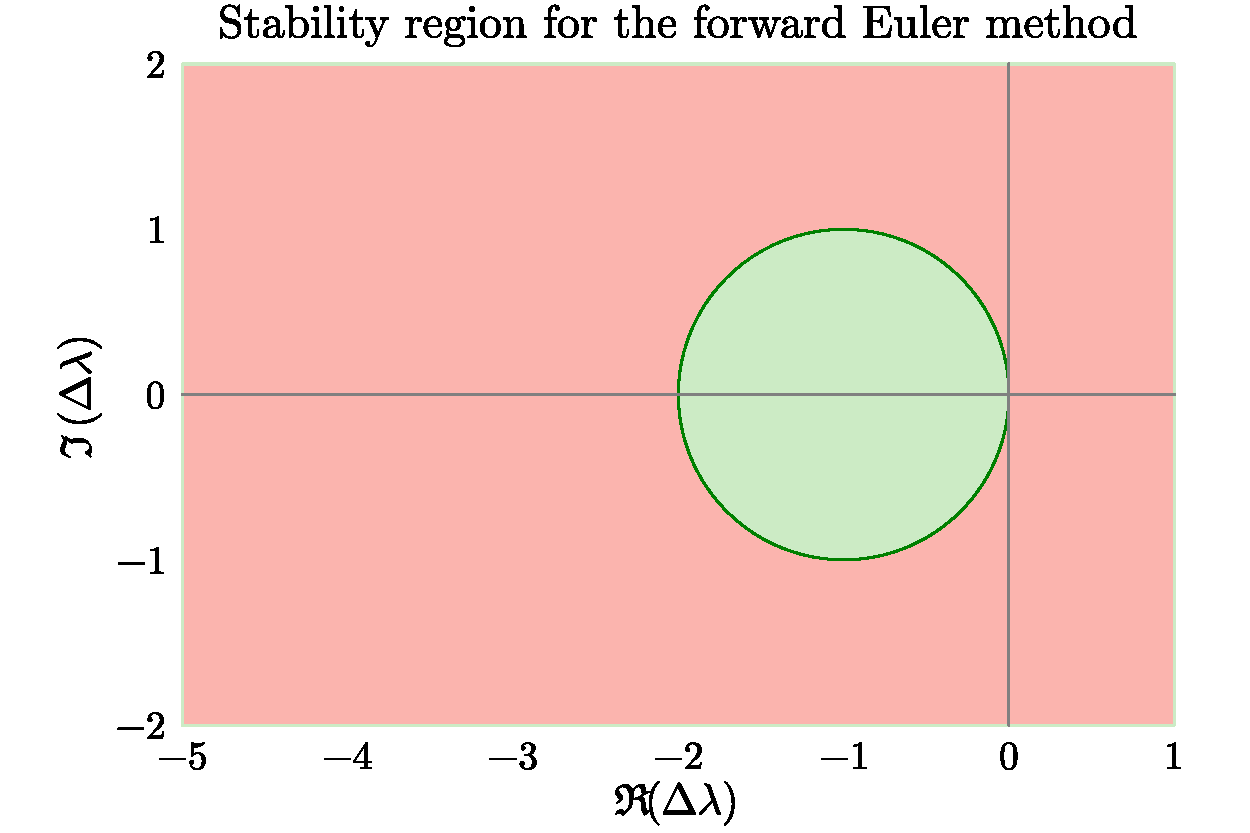
\includegraphics[width=0.49\linewidth]{figures/stability_forward Euler.pdf}
    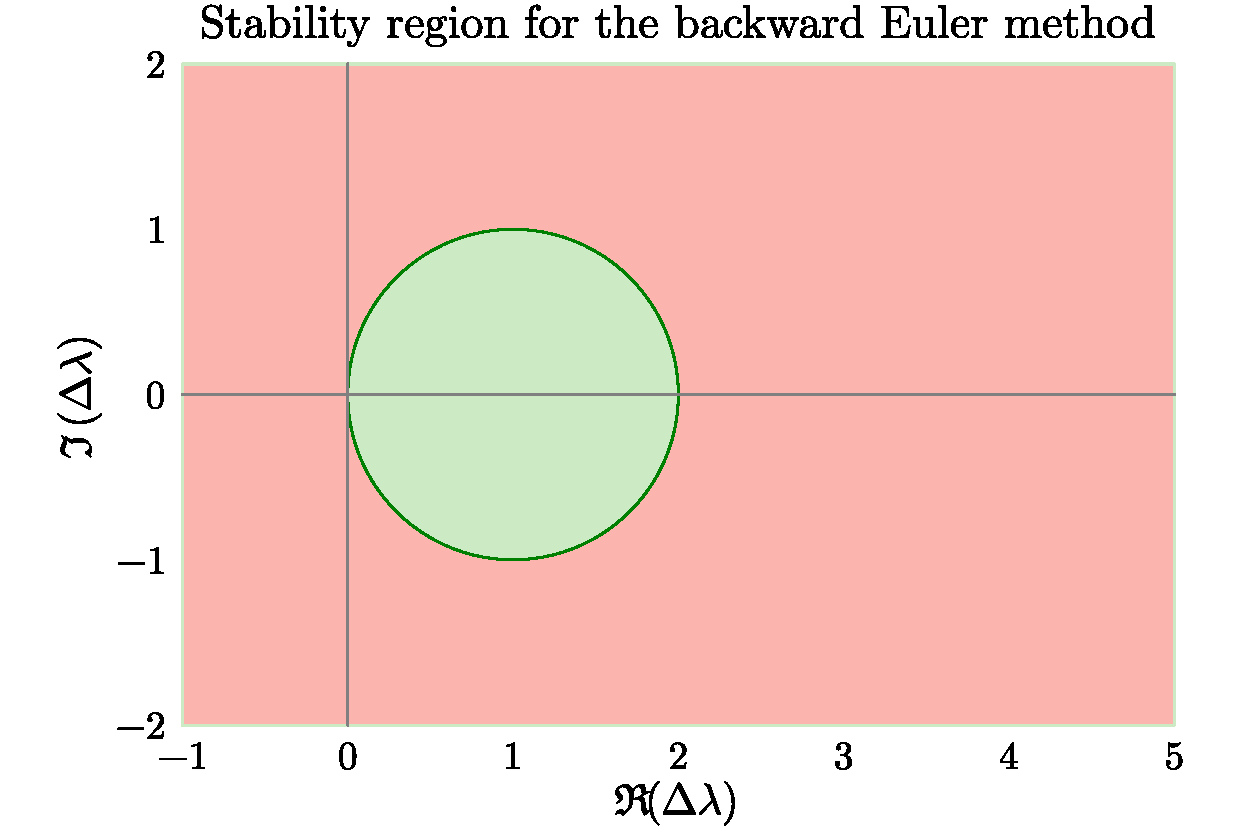
\includegraphics[width=0.49\linewidth]{figures/stability_backward Euler.pdf}
    \caption{Absolute stability regions for the forward (left) and backward (right) Euler methods.}%
    \label{fig:stab_region_euler}
\end{figure}

\begin{example}
    [Absolute stability region of the Taylor methods]
    When applied to~\eqref{eq:model_equation},
    the Taylor method of order~$p$ given in~\eqref{eq:taylor_scheme} reads
    \[
        x_{n+1} = \left(1 + \Delta \lambda + \frac{\Delta^2 \lambda^2}{2} + \dotsb + \frac{\Delta^p \lambda^p}{p!} \right) x_n.
    \]
    Thus, the absolute stability region is given by
    \[
        \left\{ z \in \complex : \left\lvert 1 + z + \frac{z^2}{2} + \dotsb + \frac{z^p}{p!} \right\rvert < 1 \right\}.
    \]
    This region is illustrated for various values of~$p$ in~\cref{fig:stab_taylor}.
    We observe that the absolute stability region grows as $p$ increases.
\end{example}

\begin{figure}[ht]
    \centering
    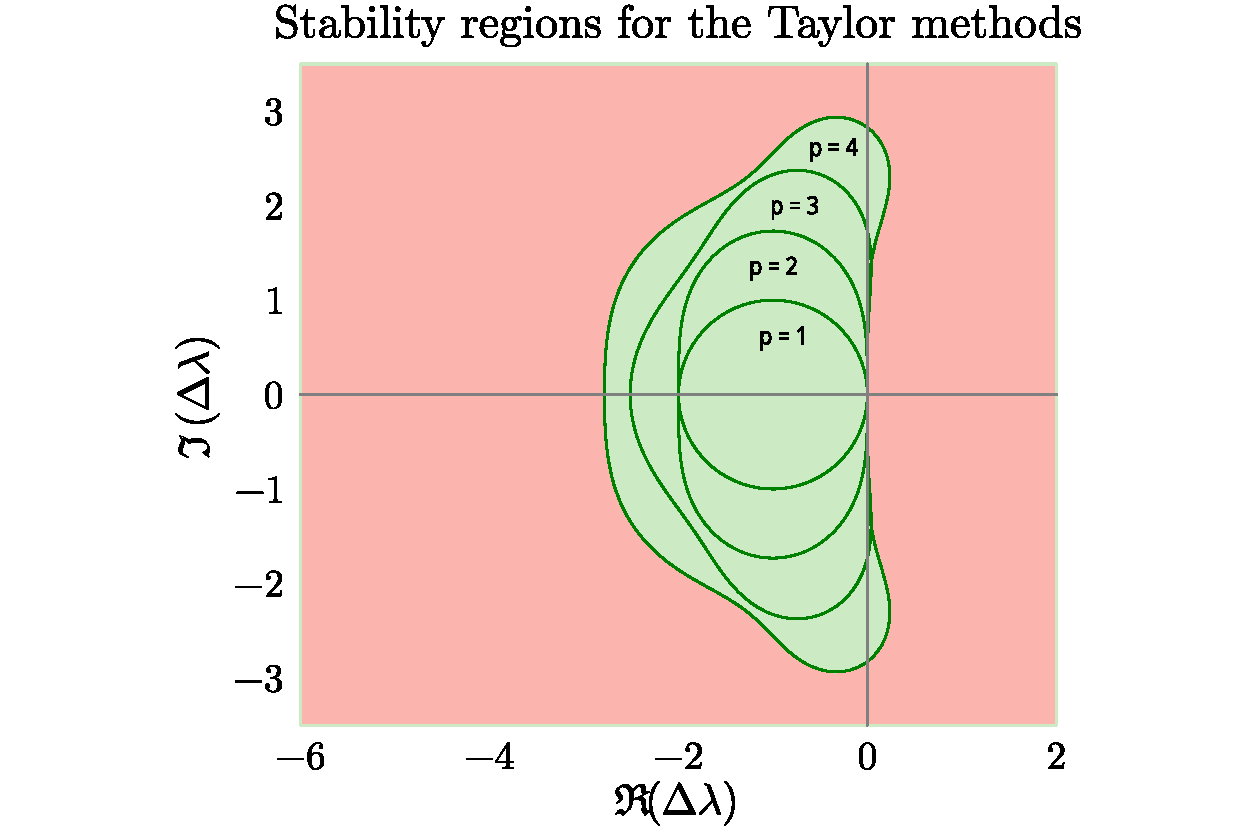
\includegraphics[width=0.70\linewidth]{figures/stability_Taylor_methods.pdf}
    \caption{Stability regions for the first few Taylor methods.}%
    \label{fig:stab_taylor}
\end{figure}

\subsection*{Stiff differential equations}
In the context of ordinary differential equations,
stiffness is not a precisely defined concept,
but rather rather a generic term employed to describe equations with widely separated time scales.
Roughly speaking, a differential equation of the form~\eqref{eq:ode} is called stiff if the Jacobian matrix of~$f$,
with respect to the variable~$\vect x$,
has at least one eigenvalue with a large negative real part.
In the one-dimensional setting,
the solutions to stiff differential equations which are close at the initial time tend to converge quickly to each other,
in view of~\eqref{eq:ode_error_equation}.
This is illustrated in~\cref{example:stiff_ode}.

\begin{example}
    [Stiff differential equation]
    \label{example:stiff_ode}
    Consider the following equation~\cite[Chapter 4]{Legat}:
    \begin{equation}
        \label{eq:stiff_ode}
        \left\{
        \begin{aligned}
            x'(t) &= - \alpha \bigl(x(t) - \sin(t) \bigr) + \cos(t) \\
            x(0) &= x_0
        \end{aligned}
        \right.
    \end{equation}
    The exact solution to this equation is given by
    \[
        x(t) = \sin(t) + x_0 \, \e^{-\alpha t}.
    \]
    When $\alpha \in \real$ is large,
    the distance between the solution and the function $t \mapsto \sin(t)$ converges to zero very quickly,
    regardless of the initial condition.
    This behavior is illustrated in~\cref{fig:stiff_ode}.
\end{example}
\begin{figure}[ht]
    \centering
    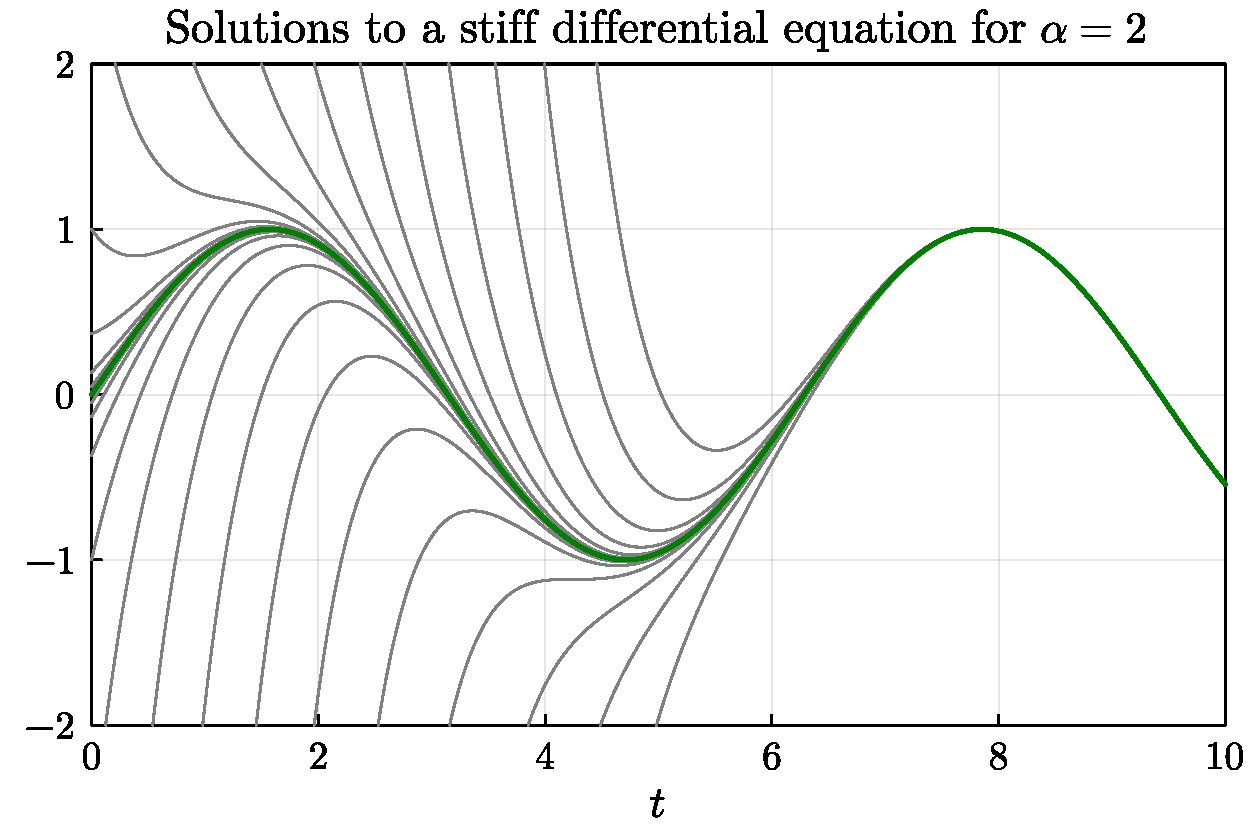
\includegraphics[width=0.49\linewidth]{figures/ode_stiff_2.pdf}
    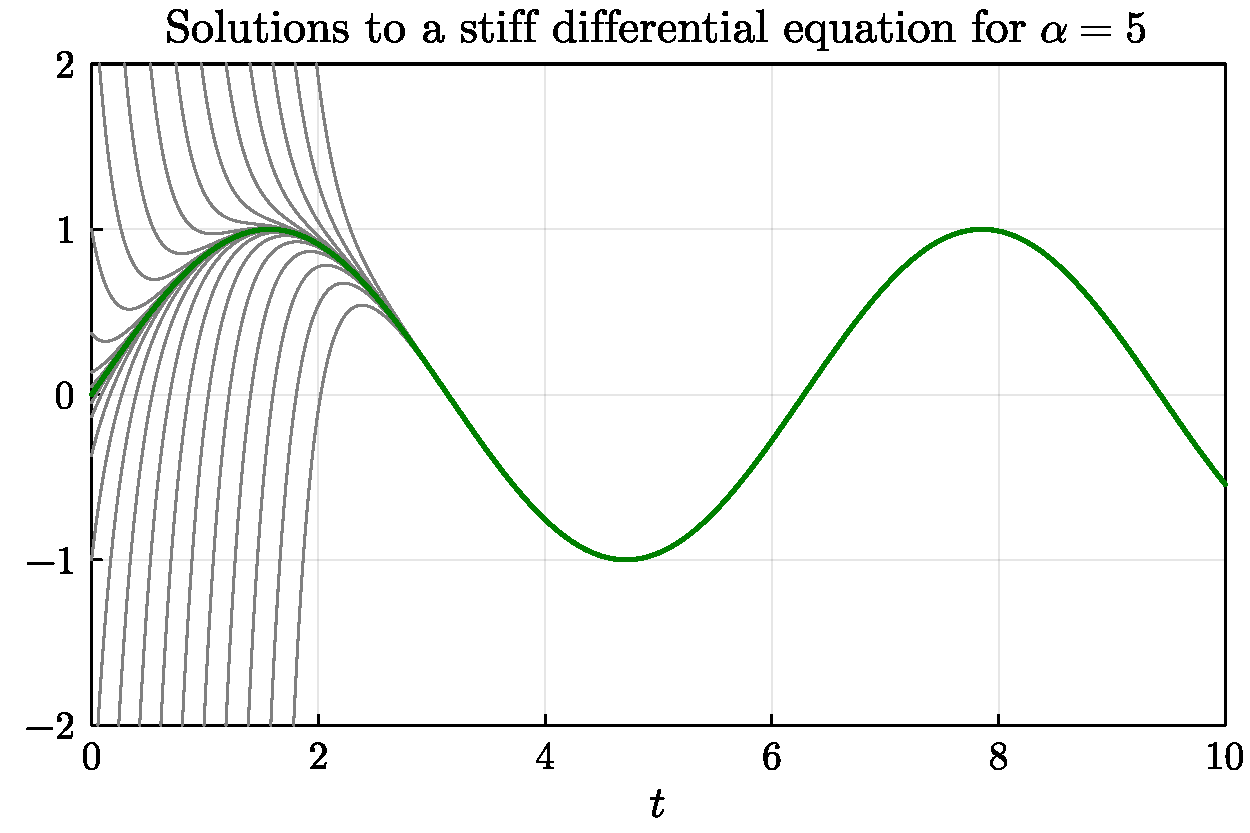
\includegraphics[width=0.49\linewidth]{figures/ode_stiff_5.pdf}
    \caption{Solutions to~\eqref{eq:stiff_ode} for various initial conditions when $\alpha = 2$ (left) and $\alpha = 5$ (right).}%
    \label{fig:stiff_ode}
\end{figure}

In the rest of this section,
we use the differential equation~\eqref{eq:stiff_ode} as a guiding example.
For this problem, we have $\partial_x f(t, x) = \alpha$.
Therefore, in view of~\eqref{eq:stability_nonlinear},
we expect that the forward Euler scheme is non-divergent if $|1 - \alpha \Delta| < 1$,
i.e.\ if
\[
    \Delta < \Delta_* ~= \frac{2}{\alpha}.
\]
It turns out that this prediction is precise,
as depicted in~\cref{fig:forward_euler_stiff}.
Note that if the equation is very stiff,
that is to say if $\alpha \gg 1$,
then a very small time step is required to ensure stability.

In contrast with the forward Euler scheme,
the backward Euler scheme is stable regardless of the time step.
Since the right-hand side of~\eqref{eq:stiff_ode} is linear in~$x$,
the value of the iterate~$x_{n+1}$ can be calculated explicitly from~$x_n$ for the backward scheme:
\[
    x_{n+1} = \frac{x_n + \Delta \alpha \sin(t_{n+1}) + \Delta \cos(t_{n+1})}{1 + \Delta \alpha}.
\]
Numerical approximations obtained using this scheme are illustrated in~\cref{fig:backward_euler_stiff}.
We observe that the method is stable even for the large time step $\Delta = 2 \Delta_*$.

\begin{figure}[ht]
    \centering
    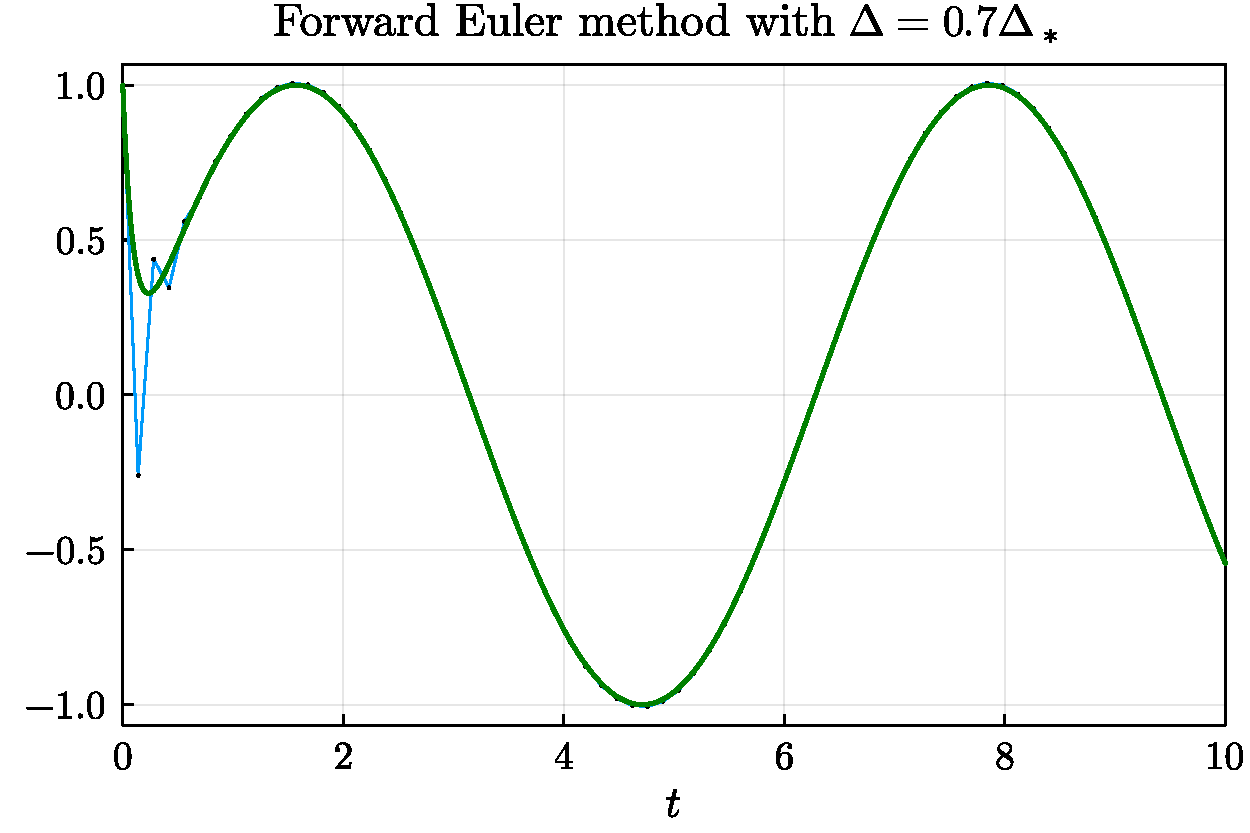
\includegraphics[width=0.48\linewidth]{figures/stiff_forward_euler_0_7.pdf}
    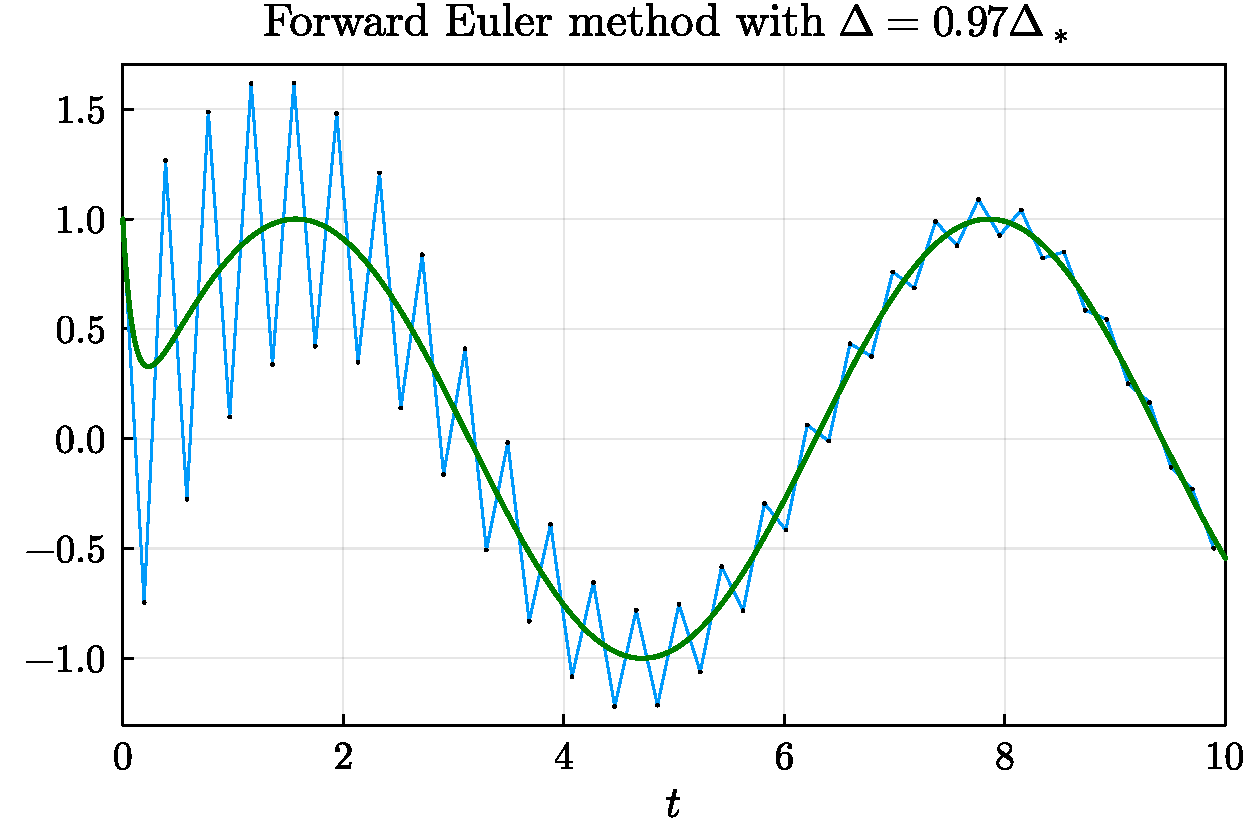
\includegraphics[width=0.48\linewidth]{figures/stiff_forward_euler_0_97.pdf}
    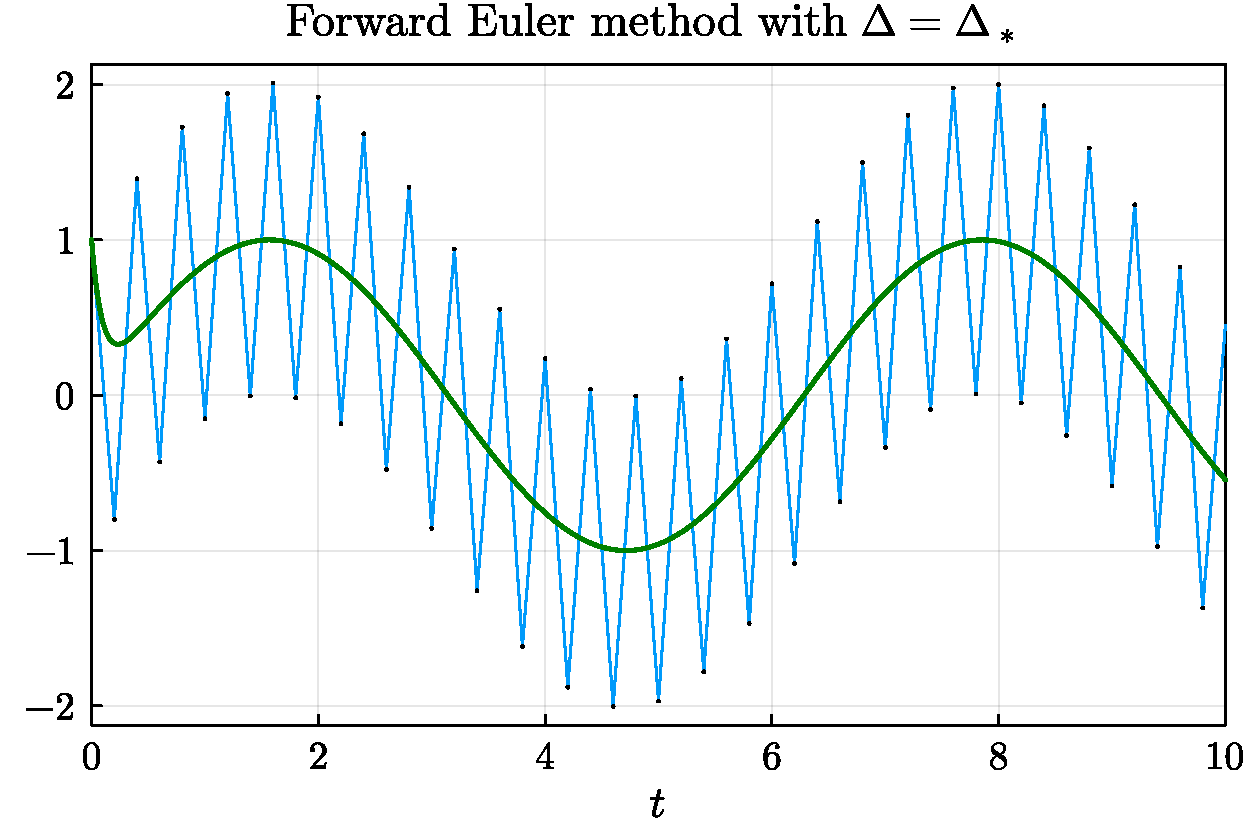
\includegraphics[width=0.48\linewidth]{figures/stiff_forward_euler_1_00.pdf}
    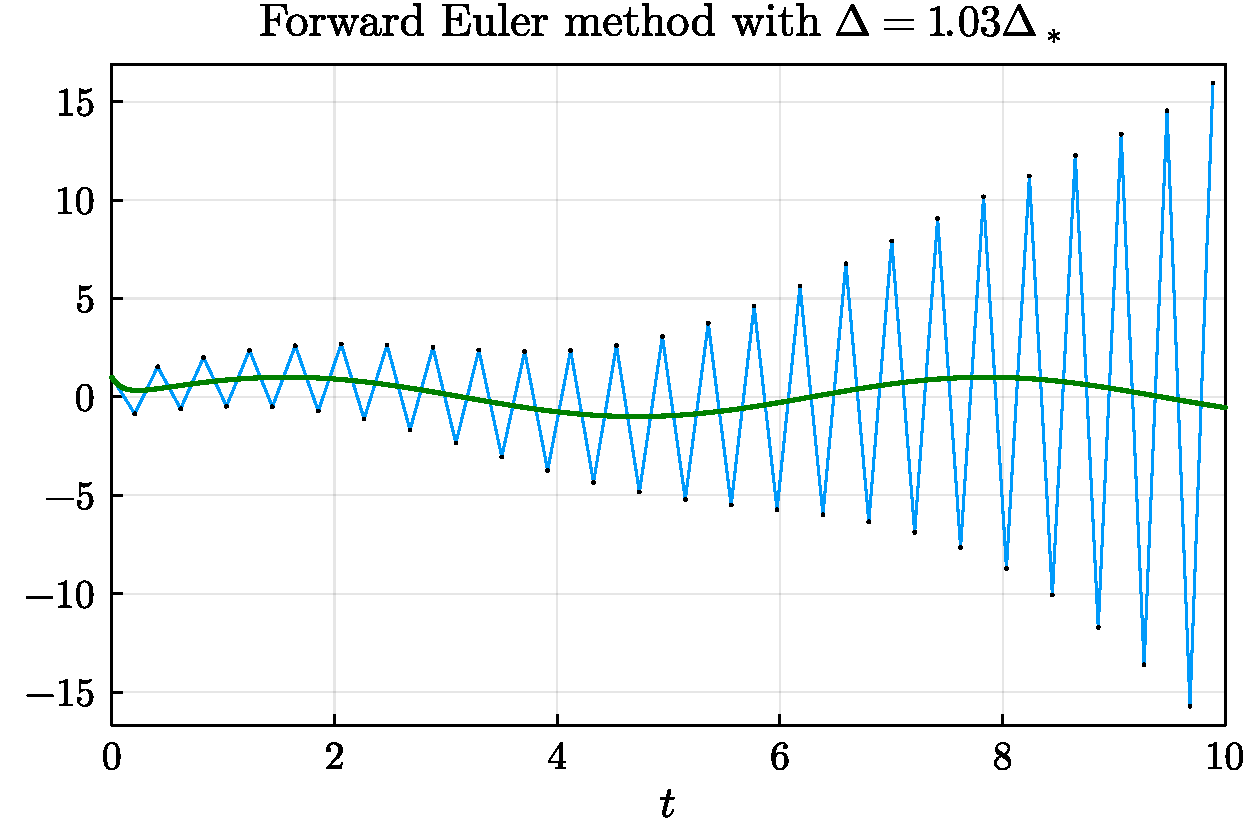
\includegraphics[width=0.48\linewidth]{figures/stiff_forward_euler_1_03.pdf}
    \caption{%
        Numerical approximations of the solution to~\eqref{eq:stiff_ode} with $\alpha = 10$ obtained with the forward Euler method,
        for four different values of $\Delta$.
    }%
    \label{fig:forward_euler_stiff}
\end{figure}

\begin{figure}[ht]
    \centering
    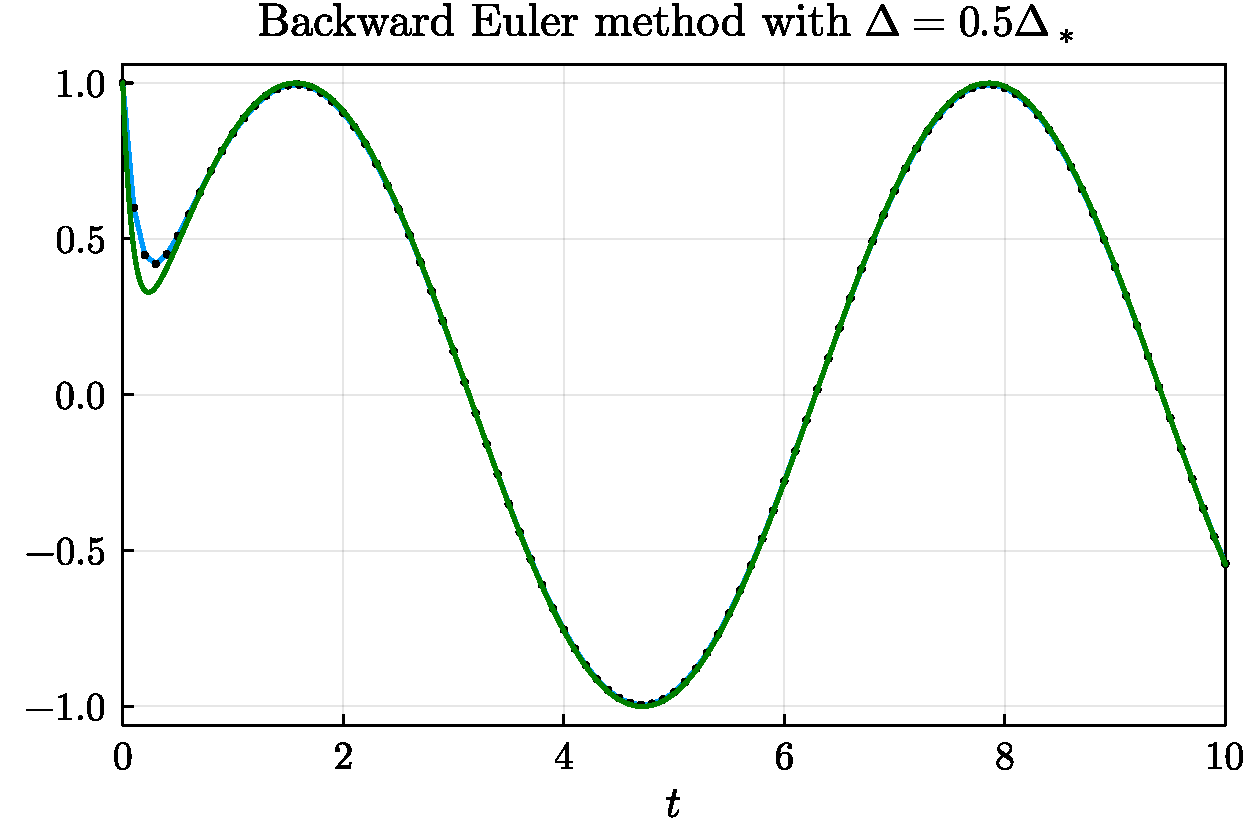
\includegraphics[width=0.48\linewidth]{figures/stiff_backward_euler_0_5.pdf}
    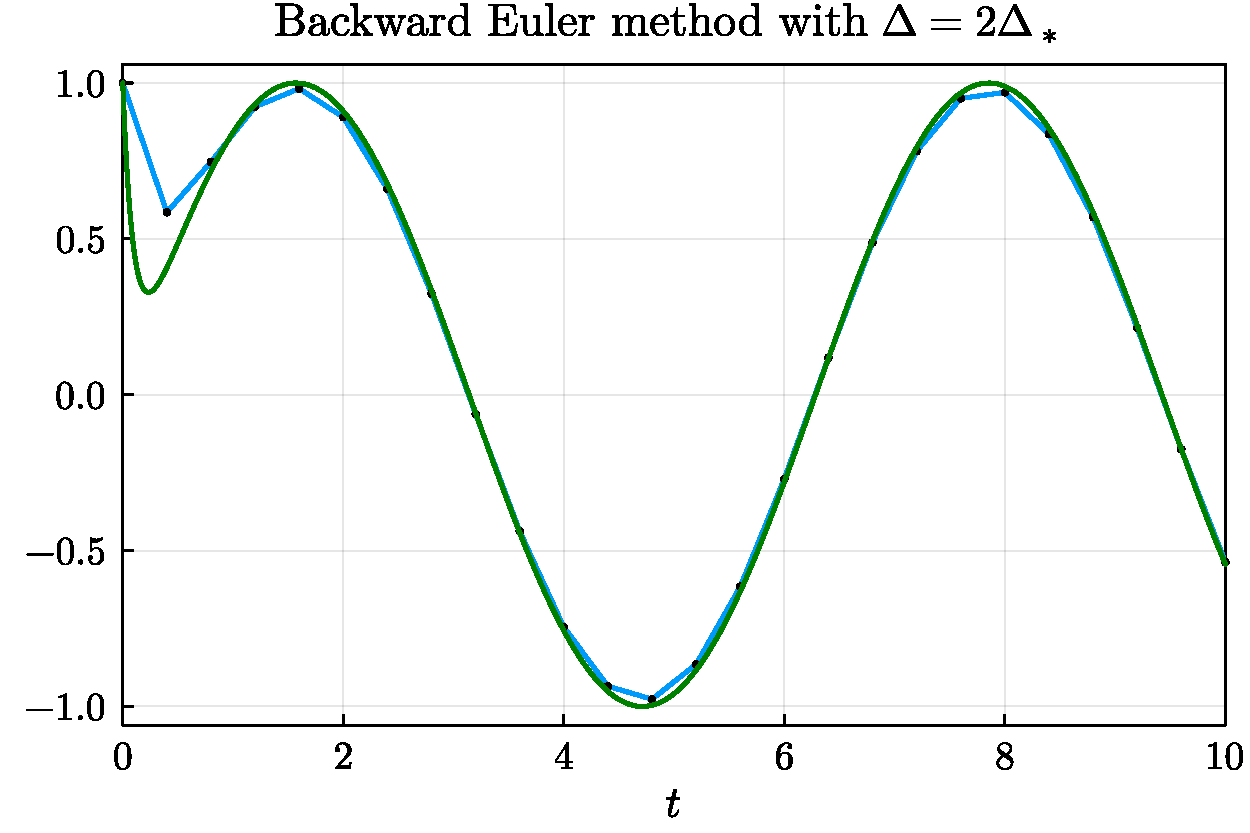
\includegraphics[width=0.48\linewidth]{figures/stiff_backward_euler_2_0.pdf}
    \caption{%
        Numerical approximations of the solution to~\eqref{eq:stiff_ode} with $\alpha = 10$ obtained with the backward Euler method,
        for two different values of $\Delta$.
    }%
    \label{fig:backward_euler_stiff}
\end{figure}
\section{Exercises}

\begin{exercise}
    Show that the absolute stability region of the Crank--Nicolson method~\eqref{eq:crank_nicolson} is given by the left half-plane;
    see~\cref{fig:stab_region_crank_nicolson}.
\end{exercise}

\begin{figure}[ht]
    \centering
    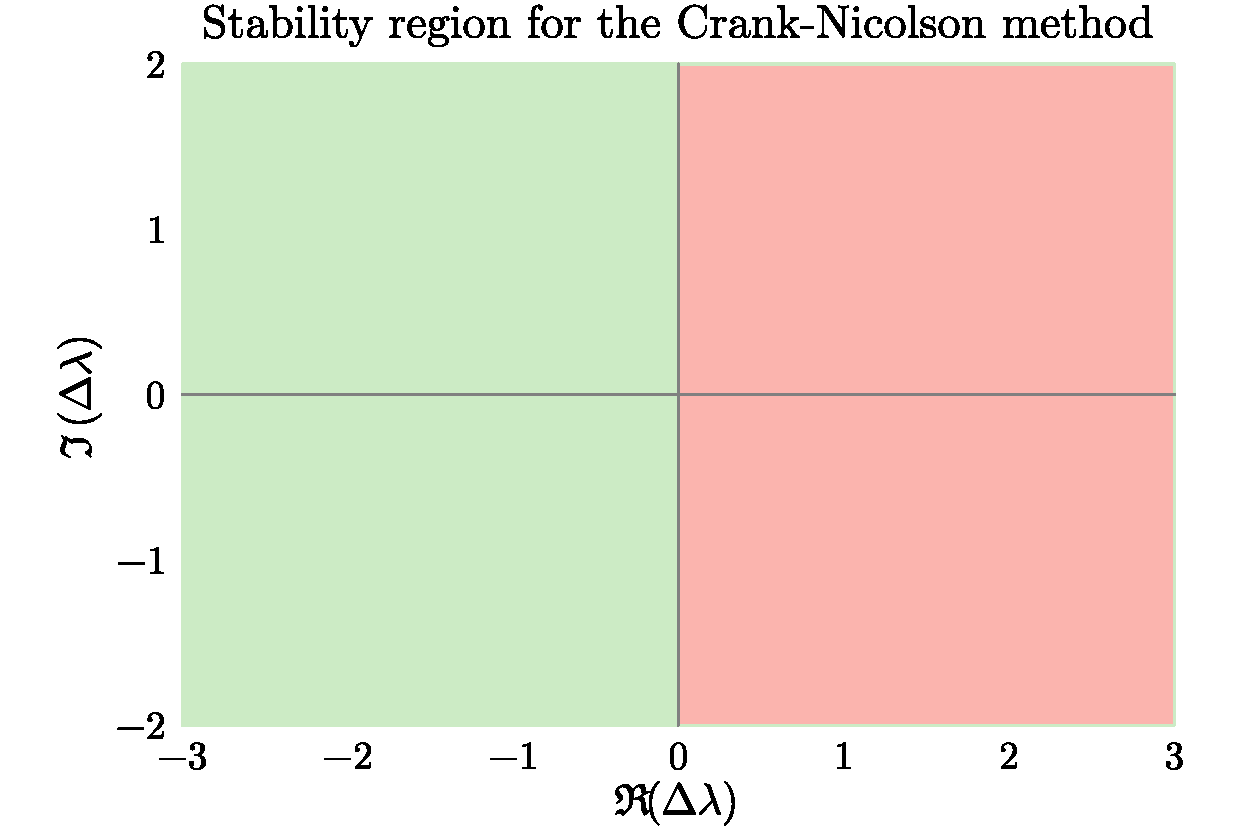
\includegraphics[width=0.7\linewidth]{figures/stability_Crank-Nicolson.pdf}
    \caption{Absolute stability regions for the Crank Nicolson method.}%
    \label{fig:stab_region_crank_nicolson}
\end{figure}

\begin{exercise}
    Calculate the absolute stability region for Gear's method.
\end{exercise}
